\documentclass[notes,11pt, aspectratio=169]{beamer}

\usepackage{pgfpages}
% These slides also contain speaker notes. You can print just the slides,
% just the notes, or both, depending on the setting below. Comment out the want
% you want.
\setbeameroption{hide notes} % Only slide
%\setbeameroption{show only notes} % Only notes
%\setbeameroption{show notes on second screen=right} % Both

%\usepackage{helvet}
%\usepackage[default]{lato}
\usepackage[T1]{fontenc}
\usefonttheme{serif}
\usefonttheme{professionalfonts}
\usepackage{tgpagella}
\usepackage{array}
\usepackage{caption}
\usepackage[labelfont={color=blue}]{caption}
\usepackage{subcaption}
\usepackage{natbib}

\usepackage{tikz}
\usepackage{verbatim}
\setbeamertemplate{note page}{\pagecolor{yellow!5}\insertnote}
\usetikzlibrary{positioning}
\usetikzlibrary{snakes}
\usetikzlibrary{calc}
\usetikzlibrary{arrows}
\usetikzlibrary{decorations.markings}
\usetikzlibrary{shapes.misc}
\usetikzlibrary{matrix,shapes,arrows,fit,tikzmark}
\usepackage{amsmath}
\usepackage{mathpazo}
\usepackage{hyperref}
\usepackage{lipsum}
\usepackage{multimedia}
\usepackage{graphicx}
\usepackage{multirow}
\usepackage{graphicx}
\usepackage{dcolumn}
\usepackage{bbm}
\newcolumntype{d}[0]{D{.}{.}{5}}

\usepackage{changepage}
\usepackage{appendixnumberbeamer}
\newcommand{\beginbackup}{
   \newcounter{framenumbervorappendix}
   \setcounter{framenumbervorappendix}{\value{framenumber}}
   \setbeamertemplate{footline}
   {
     \leavevmode%
     \hline
     box{%
       \begin{beamercolorbox}[wd=\paperwidth,ht=2.25ex,dp=1ex,right]{footlinecolor}%
%         \insertframenumber  \hspace*{2ex} 
       \end{beamercolorbox}}%
     \vskip0pt%
   }
 }
\newcommand{\backupend}{
   \addtocounter{framenumbervorappendix}{-\value{framenumber}}
   \addtocounter{framenumber}{\value{framenumbervorappendix}} 
}


\usepackage{graphicx}
\usepackage[space]{grffile}
\usepackage{booktabs}

% For tables and hidding columns
\usepackage{adjustbox}
\usepackage{threeparttable}
\newcolumntype{H}{>{\setbox0=\hbox\bgroup}c<{\egroup}@{}}

\def\sym#1{\ifmmode^{#1}\else\(^{#1}\)\fi}

% These are my colors -- there are many like them, but these ones are mine.
\definecolor{blue}{RGB}{0,69,134}
\definecolor{red}{RGB}{197,0,11}
\definecolor{yellow}{RGB}{255,211,0}
\definecolor{green}{RGB}{87,157,28}

\hypersetup{
  colorlinks = true,
  linkbordercolor = {white},
  linkcolor = {blue},
  citecolor = {red}
}


%% I use a beige off white for my background
\definecolor{MyBackground}{RGB}{255,253,218}

%% Uncomment this if you want to change the background color to something else
%\setbeamercolor{background canvas}{bg=MyBackground}

%% Change the bg color to adjust your transition slide background color!
\newenvironment{transitionframe}{
  \setbeamercolor{background canvas}{bg=blue}
  \begin{frame}}{
    \end{frame}
}

\setbeamercolor{frametitle}{fg=blue}
\setbeamercolor{title}{fg=black}
\setbeamertemplate{footline}[frame number]
\setbeamertemplate{navigation symbols}{} 
\setbeamertemplate{itemize items}{-}
\setbeamercolor{itemize item}{fg=blue}
\setbeamercolor{itemize subitem}{fg=blue}
\setbeamercolor{enumerate item}{fg=blue}
\setbeamercolor{enumerate subitem}{fg=blue}
\setbeamercolor{button}{bg=MyBackground,fg=blue,}



% If you like road maps, rather than having clutter at the top, have a roadmap show up at the end of each section 
% (and after your introduction)
% Uncomment this is if you want the roadmap!
 \AtBeginSection[]
 {
    \begin{frame}
        \frametitle{Roadmap of Talk}
        \tableofcontents[currentsection]
    \end{frame}
 }
\setbeamercolor{section in toc}{fg=blue}
\setbeamercolor{subsection in toc}{fg=red}
\setbeamersize{text margin left=1em,text margin right=1em} 

% \newenvironment{itemize}{\itemize\addtolength{\itemsep}{10pt}}{\enditemize}

\usepackage{environ}
\NewEnviron{videoframe}[1]{
  \begin{frame}
    \vspace{-8pt}
    \begin{columns}[onlytextwidth, T] % align columns
      \begin{column}{.58\textwidth}
        \begin{minipage}[t][\textheight][t]
          {\dimexpr\textwidth}
          \vspace{8pt}
          \hspace{4pt} {\Large \sc \textcolor{blue}{#1}}
          \vspace{8pt}
          
          \BODY
        \end{minipage}
      \end{column}%
      \hfill%
      \begin{column}{.42\textwidth}
        \colorbox{green!20}{\begin{minipage}[t][1.2\textheight][t]
            {\dimexpr\textwidth}
            Face goes here
          \end{minipage}}
      \end{column}%
    \end{columns}
  \end{frame}
}

\title[]{\textcolor{blue}{The long-term effects of attending an elite high-school}}
\author[Marco Medina]{}
\institute[FRBNY]{\small{\begin{tabular}{c c c c c}
Mauricio Romero &&  Enrique Seira && Rafael de Hoyos   \\
ITAM && ITAM/MSU && World Bank \\ \\

\end{tabular}}}

\date{UCSD-ITAM Workshop \\ March 11th, 2023}


\begin{document}

%%% TIKZ STUFF
\tikzset{   
        every picture/.style={remember picture,baseline},
        every node/.style={anchor=base,align=center,outer sep=1.5pt},
        every path/.style={thick},
        }
\newcommand\marktopleft[1]{%
    \tikz[overlay,remember picture] 
        \node (marker-#1-a) at (-.3em,.3em) {};%
}
\newcommand\markbottomright[2]{%
    \tikz[overlay,remember picture] 
        \node (marker-#1-b) at (0em,0em) {};%
}
\tikzstyle{every picture}+=[remember picture] 
\tikzstyle{mybox} =[draw=black, very thick, rectangle, inner sep=10pt, inner ysep=20pt]
\tikzstyle{fancytitle} =[draw=black,fill=red, text=white]
%%%% END TIKZ STUFF

% Title Slide
\begin{frame}
\maketitle
  % \centering The views expressed do not necessarily reflect the position of Somewhere Fancy.
\end{frame}

\begin{frame}[fragile]{Motivation}
  \begin{itemize}[<+->]
    \vfill\item Most cities/countries have schools that are deemed ``elite'' (high demand)
    \vfill\item Mostly, these schools \text{do not} have better ``value-added'' in terms of academic outcomes for the marginal applicant \tiny{\citep{Adrienne2014,ElliteIllusion,DobbieFryer2014,dustan2017flourish,ParentsValueEffectiveness}}
\vfill\item What drives demand for these schools?
  \begin{itemize}
    \vfill\item Maybe they have effects on labor market outcomes?
      \begin{itemize}
     \vfill\item Peer composition does changes \tiny{\citep{ElliteIllusion,DobbieFryer2014,ParentsValueEffectiveness}}
       \end{itemize}
    \vfill\item Maybe current RD estimates do not reflect treatment effects for most applicants
  \end{itemize}
    \end{itemize}
\end{frame}

\begin{frame}[fragile]{This paper}
  \begin{itemize}
    \vfill\item Estimate the effects of attending an ``elite'' school on labor market outcomes, voting behavior, and migration/location
    \vfill\item Estimate heterogeneity in treatment effects by student characteristics
    \end{itemize}
\end{frame}


% \begin{frame}[fragile]{Aim: where does this paper fit?}
%   \begin{itemize}
%     \vfill\item \citet{Estrada2017,dustan2017flourish} have looked into the short-term effects of being assigned to an elite (IPN) school. We aim to look into long-term effects.
%     \vfill\item \citet{abdulkadirouglu2011accountability}, \citet{deming2011better}, \citet{deming2014school} and \citet{angrist2017leveraging} have exploited the random assignment of first choices. We aim to exploit the whole list of requested schools as in \citet{abdulkadirouglu2022breaking}.
%     \vfill\item \textcolor{yellow}{Cite papers about DA and school type} have looked into the effect of a type of school (e.g. charter schools). We aim to look into the value added affect of each school \textcolor{yellow}{Cite papers about VAM, Kirabo}.
%     \vfill\item Most papers focus on the LATE obtained at the discontinuity resulting in random assignment. We aim to estimate the marginal treatment effect distribution at each school exploiting the ``cutoffs'' for the next best option of each applicant. \citep{Kowalski,Kowalski2021,NBERw22363}.
%   \end{itemize}
% \end{frame}



\section{Context}


\begin{frame}[fragile]{Context}
  \begin{itemize}
    \vfill\item Admissions to public high schools in the Greater Mexico City area are centralized.
    \vfill\item Admissions managed by the Metropolitan Commission of Public Senior-Secondary Education Institutions (COMIPEMS).
    \vfill\item Applicants take an exam and submit preferences to different schools each year. 
    \vfill\item The allocation mechanism is \textcolor{red}{serial dictatorship}. 
  \end{itemize}
\end{frame}

\begin{frame}[fragile]{Admission mechanism: Serial dictatorship}
  \begin{itemize}
    \vfill\item In February, students submit their ranked preferences (up to 20 schools).
    \vfill\item In June, students take a comprehensive exam (math, Spanish science, social studies).
    \begin{itemize}
    \vfill\item Commonly known as the COMIPEMS exam.
    \end{itemize}
    \vfill\item Students are ordered according to their exam score.
      \begin{itemize}
    \vfill\item Schools do not have any other preference over students.
    \end{itemize}
    \vfill\item Starting with the highest scores, students are assigned to their highest-ranking school with available seats.
  \end{itemize}
\end{frame}

\begin{frame}[fragile]{Admission mechanism: Side note}
  \begin{itemize}
    \vfill\item There are multiple test centers 
    \vfill\item Students are assigned to test centers based on:
      \begin{itemize}
    \vfill\item Where they live
    \vfill\item The first letter of their last name
    \vfill\item The date they enter their application
    \vfill\item If their top choice is an UNAM school
     \end{itemize}
     \vfill\item Conditional on the previous conditions, assignment is random
     \vfill\item Separate paper: effects of pollution on the day of the test
  \end{itemize}
\end{frame}


\begin{frame}[fragile]{High-school types and subsystems}
  \begin{itemize}
    \vfill\item The 361 public schools in Mexico City are managed by nine entities.
    
\vfill\item 222 schools managed by 4 entities offer \textcolor{red}{traditional} high-school education 
  \begin{itemize}
\vfill\item Colegio de Bachilleres (COLBACH) $\rightarrow$ 20 schools
\vfill\item Secretaría de Educación del
Gobierno del Estado de México (SE) $\rightarrow$ 199 schools
\vfill\item Dirección General del Bachillerato (DGB) $\rightarrow$ 2 schools
\vfill\item Universidad Autónoma del Estado de México (UAEM) $\rightarrow$ 1 school
  \end{itemize}  
    \vfill\item 109 schools managed by 3 entities manage \textcolor{red}{vocational} schools
  \begin{itemize}
\vfill\item Colegio Nacional de Educación Profesional Técnica (CONALEP) $\rightarrow$ 57 schools
\vfill\item Dirección General de Educación Tecnológica Agropecuaria (DGETA)  $\rightarrow$ 1 school
\vfill\item Dirección General de Educación Tecnológica Industrial (DGETI)  $\rightarrow$ 51 schools
  \end{itemize}  

    \vfill\item 30 schools managed by 2 entities are considered \textcolor{red}{elite}
      \begin{itemize}
    \vfill\item Universidad Nacional Autónoma de México (UNAM) $\rightarrow$ 14  schools. 
    \vfill\item Instituto Politécnico Nacional (IPN) $\rightarrow$ 16 schools.
  \end{itemize} 

    
  \end{itemize}
\end{frame}

\begin{frame}{High-school types and subsystems map}
    \centering
    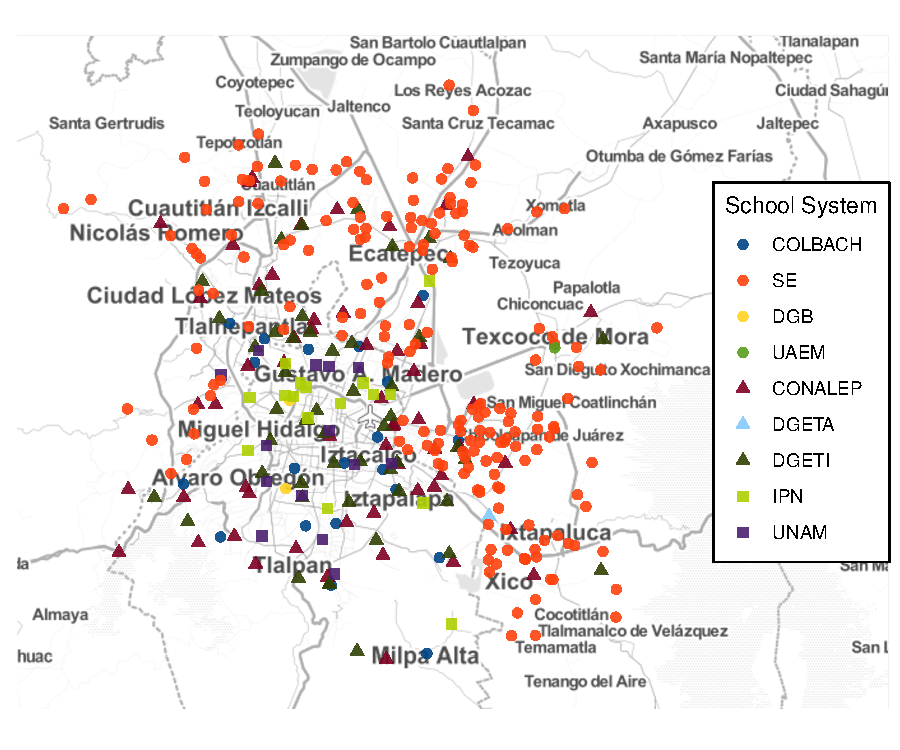
\includegraphics[width=0.65\textwidth]{04_Figures/comipems_type_map_ggmap.pdf}
\end{frame}

% \begin{frame}[fragile]{High-school types and subsystems}
%   \begin{itemize}
%     \item There are three subsystems that focus on vocational and technical training. 
%     \item These includes schools include those ran by Colegio Nacional de Educación Profesional Técnica (CONALEP), Dirección General de Educación Tecnológica Agropecuaria (DGETA), and Dirección General de Educación Tecnológica Industrial (DGETI).
%     \item The remaining four subsystems offer traditional high-school education, and are not considered elite: Colegio de Bachilleres (COLBACH), Secretaría de Educación del Gobierno del Estado de México (SE), Dirección General del Bachillerato (DGB), and Universidad Autónoma del Estado de México (UAEM).
%   \end{itemize}
% \end{frame}



\section{Data}



\begin{frame}{COMIPEMS data}
  \begin{itemize}
    \vfill\item We have data on 6 cohorts of applicants (2005-2010).
    \vfill\item For each applicant
      \begin{itemize}
      \vfill\item National identifier (CURP)
      \vfill\item Zip code of residence
      \vfill\item DOB and gender
      \vfill\item Middle school they attend (and GPA)
      \vfill\item Where they are tested
      \vfill\item Test score
      \vfill\item Ordered list of schools
      \vfill\item Assigned school
      \end{itemize}
          \vfill\item For each school, we can calculate the implied  cutoff.
  \end{itemize}
    
\end{frame}

\begin{frame}{Summary statistics}
\begin{table}[H]
\centering
\begin{adjustbox}{totalheight=0.9\textheight}
\begin{threeparttable}
\centering
%\caption{Balance across those assigned to either IPN high-school, and those who are not\label{tab:Balance_IPN}}
\begin{tabular}[t]{@{}l}
\toprule
\begin{tabular}[t]{lcccccc}
&	\multicolumn{6}{c}{Cohort} \\
 \cmidrule(lr){2-7}
                    &\multicolumn{1}{c}{2005}&\multicolumn{1}{c}{2006}&\multicolumn{1}{c}{2007}&\multicolumn{1}{c}{2008}&\multicolumn{1}{c}{2009}&\multicolumn{1}{c}{2010}\\
\hline
Num. requested schools&        8.76         &        9.17         &        9.32         &        9.55         &        9.58         &        9.76         \\
                    &      (3.62)         &      (3.67)         &      (3.75)         &      (3.74)         &      (3.71)         &      (3.82)         \\
[1em]
Test score (\%)     &        0.50         &        0.51         &        0.51         &        0.52         &        0.49         &        0.51         \\
                    &      (0.14)         &      (0.14)         &      (0.15)         &      (0.15)         &      (0.14)         &      (0.15)         \\
[1em]
Male                &        0.49         &        0.49         &        0.49         &        0.48         &        0.49         &        0.49         \\
                    &      (0.50)         &      (0.50)         &      (0.50)         &      (0.50)         &      (0.50)         &      (0.50)         \\
[1em]
IPN assignment      &        0.08         &        0.08         &        0.08         &        0.08         &        0.08         &        0.08         \\
                    &      (0.27)         &      (0.27)         &      (0.27)         &      (0.27)         &      (0.27)         &      (0.27)         \\
[1em]
UNAM assignment     &        0.14         &        0.13         &        0.13         &        0.14         &        0.13         &        0.13         \\
                    &      (0.35)         &      (0.34)         &      (0.34)         &      (0.34)         &      (0.33)         &      (0.33)         \\
[1em]
Elite assignment    &        0.21         &        0.21         &        0.21         &        0.22         &        0.20         &        0.21         \\
                    &      (0.41)         &      (0.41)         &      (0.41)         &      (0.41)         &      (0.40)         &      (0.41)         \\
\hline
Applicants          &     249,123         &     255,456         &     255,955         &     256,772         &     266,810         &     269,776         \\

\end{tabular}
\tabularnewline \bottomrule
\end{tabular}
\end{threeparttable}
\end{adjustbox}
\end{table}
\end{frame}

\begin{frame}{Outcome data}
  \begin{itemize}
    \vfill\item Data from a standardized test students were required to take when they graduate
  \begin{itemize}
  \vfill\item Taking the exam is a good proxy for graduating (except for UNAM students)
    \vfill\item Math and Spanish scores at the end of high-school
    \vfill\item Wage expectations
    \vfill\item Aspirations
      \end{itemize}

    \vfill\item Data from The National Electoral Institute (INE) for 2012, 2015, and 2018
      \begin{itemize}
    \vfill\item If voted 
    \vfill\item Zipcode of residence 
    \vfill\item If unable to vote (due to committing a felony)
    \vfill\item Self-reported education
    \vfill\item Self-reported occupation
      \end{itemize}
  \end{itemize}
\end{frame}

\section{Empirical strategy}

\begin{frame}{Empirical strategy}
  \begin{itemize}
     \vfill\item Intuitively, we can use RD around the cutoff in each school to estimate causal effects
     \vfill\item Need to condition by preference order ($\theta_i$) to avoid omitted variables
bias

$$Y_i=\alpha 1_{s_i>c}+a(s_i,c)+\sum_{x}\gamma_{x}\theta_{i}(x)+\varepsilon_i $$
\pause

\vfill\item However, this discards much of the variation generated by the mechanism
     \vfill\item Specifically, given test scores and cutoffs, two students with different school options could have the same probability of being assigned to a school.
\vfill\item \citet{abdulkadirouglu2022breaking} show that controlling for the (local) probability of being assigned to an elite school yields unbiased estimators (and is more efficient).
  \end{itemize}
\end{frame}


% \begin{frame}{Empirical strategy}
%   \begin{itemize}
%      \vfill\item School assignment mechanisms which used DA have been used as quasi-experimental frameworks to measure causal effect of school attendance.
%      \vfill\item The first papers to use the list of requested options had their sample be the students subject to random assignment at their first choice school.
%     \vfill \item This approach fails to exploit the information contained in the ranked lists each student presents.
%      \vfill\item Specifically, given test scores and cutoffs, two students with different school options could have the same probability of being assigned to school $s$.
%      \vfill\item We follow the assignment mechanism and specification proposed by  \vfill\citet{abdulkadirouglu2022breaking}, which controls by the (local) probability of being assigned to an elite school.
%   \end{itemize}
% \end{frame}

\begin{frame}{Which cutoffs matter for assignment probabilities?}
  \begin{itemize}
  \vfill\item Define the student's type $\theta$ as the student's list of school options. Two students have the same type if they have the same school options in the same order of preference.
    \vfill\item Under serial dictatorship, the assignment probability faced by the student of type $\theta$ at school $s$ is determined by the cutoff at $s$ and by cutoffs at schools preferred to $s$.
      \begin{itemize}
    \vfill\item Since the assignment uses single tie-breaking with the test score, it is enough to know only one of cutoffs of the higher ranked schools.
    \vfill\item Failing to clear the lowest score cutoff of preferred schools to $s$ means failing all the cutoffs of the higher ranked schools.
    \vfill\item We will call the minimum cutoff of the higher ranked than $s$ schools for student of type $\theta$ the \textcolor{red}{most informative disqualification (MID)}.
     \end{itemize}
  \end{itemize}
\end{frame}

\begin{frame}{Local propensity score at school $s$}
\begin{center}
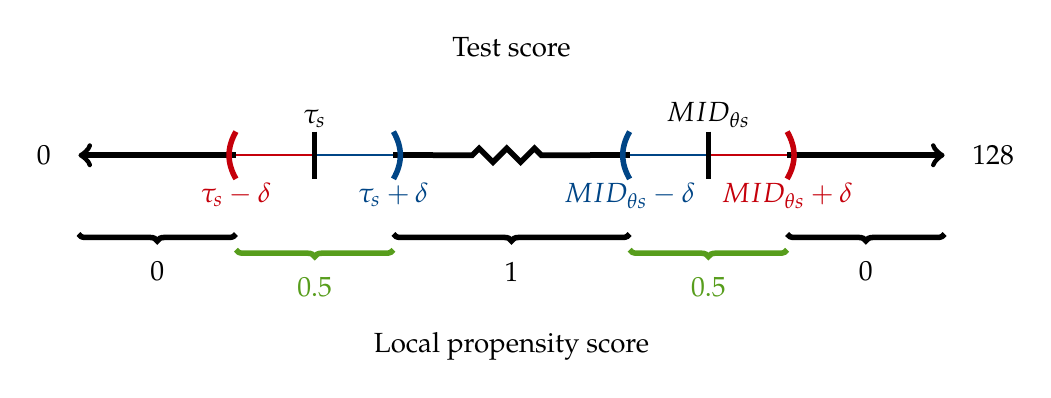
\begin{tikzpicture}[snake=zigzag, line before snake = 5mm, line after snake = 5mm, line width=2pt]
    % draw horizontal line   
    \draw [<-](-1,0) -- (1,0);
    \draw[red, thick](1,0) -- (2,0);
    \draw[blue, thick] (2,0) -- (3,0);
    \draw (3,0) -- (3.5,0);
    \draw[snake] (3.5,0) -- (5.5,0);
    \draw (5.5,0) -- (6,0);
    \draw[blue, thick](6,0) -- (7,0);
    \draw[red, thick] (7,0) -- (8,0);
    \draw[->] (8,0) -- (10,0);

    % draw vertical lines
    \foreach \x in {1}
      \draw[red] (\x cm,.3) to[bend right] (\x cm,-.3);
    \foreach \x in {8}
      \draw[red] (\x cm,.3) to[bend left] (\x cm,-.3);
    \foreach \x in {3}
      \draw[blue] (\x cm,.3) to[bend left] (\x cm,-.3);
    \foreach \x in {6}
      \draw[blue] (\x cm,.3) to[bend right] (\x cm,-.3);
    \foreach \x in {2,7}
      \draw (\x cm,.3) -- (\x cm,-.3);

    % braces
    \draw[decorate, decoration = {brace,mirror}] (-1,-1) --  (1,-1);
    \draw[green, decorate, decoration = {brace,mirror}] (1,-1.2) --  (3,-1.2);
    \draw[decorate, decoration = {brace,mirror}] (3,-1) --  (6,-1);
    \draw[green, decorate, decoration = {brace,mirror}] (6,-1.2) --  (8,-1.2);
    \draw[decorate, decoration = {brace,mirror}] (8,-1) --  (10,-1);

    % draw nodes
    \draw (1,0) node[below=.2] {\textcolor{red}{$\tau_s - \delta$}}  node[left=.105] {};
    \draw (2,0) node[above=.2] {$\tau_s$}  node[left=.105] {};
    \draw (3,0) node[below=.2] {\textcolor{blue}{$\tau_s + \delta$}}  node[left=.105] {};

    \draw (6,0) node[below=.2] {\textcolor{blue}{$MID_{\theta s} - \delta$}}  node[left=.105] {};
    \draw (7,0) node[above=.2] {$MID_{\theta s}$}  node[left=.105] {};
    \draw (8,0) node[below=.2] {\textcolor{red}{$MID_{\theta s} + \delta$}}  node[left=.105] {};

    \draw (0,-1) node[below=.2] {0};
    \draw[green] (2,-1.2) node[below=.2] {0.5};
    \draw (4.5,-1) node[below=.2] {1};
    \draw[green] (7,-1.2) node[below=.2] {0.5};
    \draw (9,-1) node[below=.2] {0};

    \draw (-1,0) node[below=.1] {}  node[left=.2] {$0$};
    \draw (10,0) node[below=.1] {}  node[right=.2] {$128$};
    \draw (4.5,1) node[above=.1] {Test score};
    \draw (4.5,-2) node[below=.1] {Local propensity score};
    
\end{tikzpicture}
\end{center}

\pause
  \begin{itemize}
  \vfill\item The sample consists of applicants for
whom the score is 0.5
\vfill\item We can now control for the local propensity score at each school
$$Y_i=\alpha 1_{s_i>c}+a(s_i,c)+\sum_{x}\gamma_{x}d_{i}(x)+\varepsilon_i $$
\end{itemize}
\end{frame}



\section{Results}


\subsection{Balance}

\begin{frame}[label=balance_rd_plot, fragile]{RD plots for balance variables}
Example of balance across those assigned to an IPN school and those who are not. \hyperlink{balance_rd_plot_app}{\beamergotobutton{Balance RD plots}}

\onslide<2-10>{
\begin{figure}
\begin{columns}[T]
\begin{column}{.5\textwidth}
\alt<6-9>{
    \begin{itemize}
        \item[]
        \item<7-> RD around the most informative disqualification (MID).
        \item<8-> Observations on the \textcolor{blue}{left } of the MID are eligible (\textcolor{blue}{treated}).
        \item<9-> Observations on the \textcolor{red}{right} are eligible at a higher ranked school (\textcolor{red}{controls}).
    \end{itemize}}
    {\begin{subfigure}{\textwidth}
        \centering
        \caption{GPA (middle school) around cutoff}
        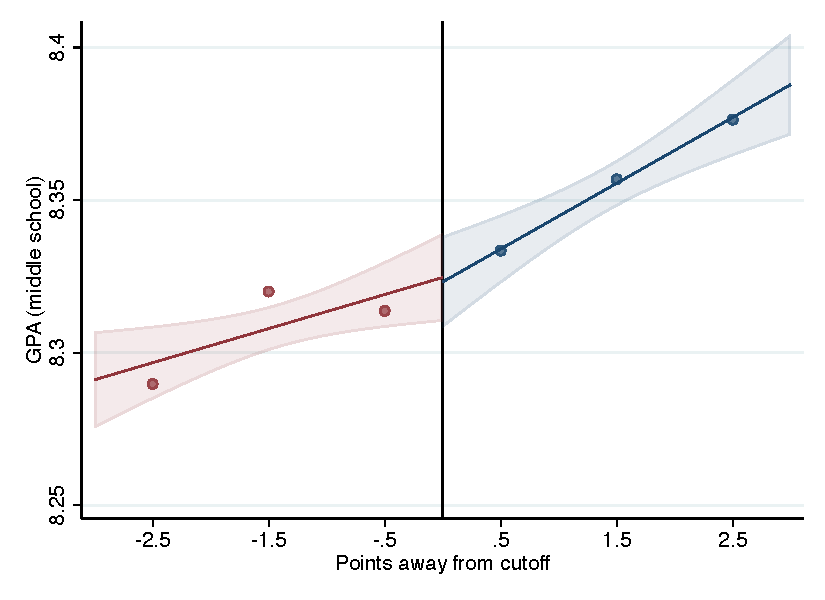
\includegraphics[width=\textwidth]{04_Figures/rd_plot_tau_sus_prom_IPN3.pdf}
    \end{subfigure}}
\end{column}

\begin{column}{.5\textwidth}
\alt<2-5>{
    \begin{itemize}
        \item[]
        \item<3-> RD around the cutoff.
        \item<4-> Observations on the \textcolor{red}{left} of the cutoff are ineligible (\textcolor{red}{controls}).
        \item<5-> Observations on the \textcolor{blue}{right} are eligible (\textcolor{blue}{treated}).
    \end{itemize}}
    {\begin{subfigure}{\textwidth}
        \centering
        \caption{GPA (middle school) plot around MID}
        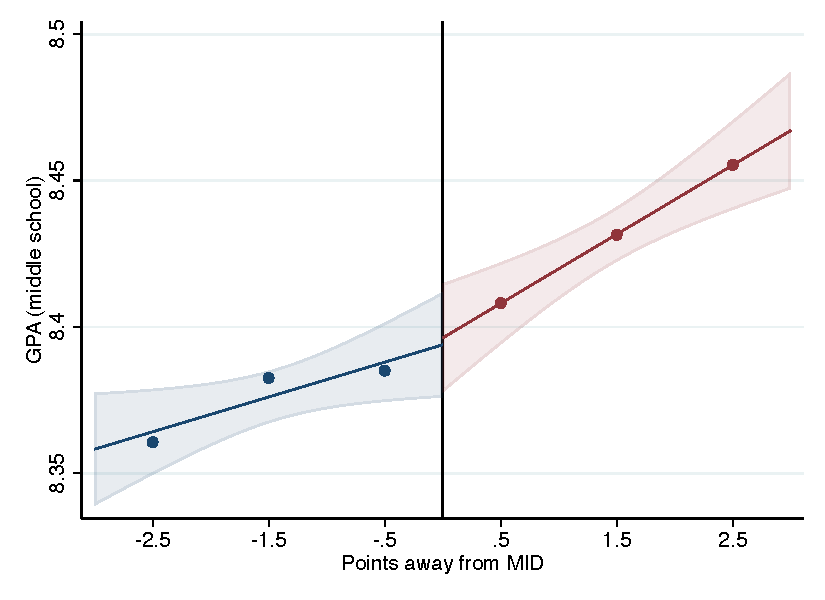
\includegraphics[width=\textwidth]{04_Figures/rd_plot_mid_sus_prom_IPN3.pdf}
    \end{subfigure}}
\end{column}
\end{columns}

\label{fig:balance_rd_plot}    
\end{figure}}

\end{frame}

\begin{frame}[fragile]{Balance across those assigned and not assigned to an IPN school}
\begin{table}[H]
\centering
\begin{adjustbox}{totalheight=0.85\textheight}
\begin{threeparttable}
\centering
%\caption{Balance across those assigned to either IPN high-school, and those who are not\label{tab:Balance_IPN}}
\begin{tabular}[t]{@{}l@{}l@{}l}
\toprule
\begin{tabular}[t]{lcc}
&	\multicolumn{2}{c}{1 point} \\
 \cmidrule(lr){2-3}
& Control &		Treatment 	\\ 
& mean & differential \\
&   (1) 	&  (2)		\\
\midrule
Age(2018)           &       25.21&       -0.01         \\
                    &      (2.09)&      (0.02)         \\
                    &     [6,206]&     [5,920]         \\
Male                &        0.54&        0.01         \\
                    &      (0.50)&      (0.01)         \\
                    &     [6,206]&     [5,920]         \\
Private (middle school)&        0.10&        0.00         \\
                    &      (0.29)&      (0.01)         \\
                    &     [6,206]&     [5,920]         \\
GPA (middle school) &        8.35&        0.00         \\
                    &      (0.77)&      (0.01)         \\
                    &     [6,206]&     [5,920]         \\
Middle school graduation&    2,007.53&       -0.00         \\
                    &      (1.93)&      (0.02)         \\
                    &     [6,206]&     [5,920]         \\
Father's age        &        4.19&       -0.03         \\
                    &      (1.55)&      (0.03)         \\
                    &     [4,801]&     [4,617]         \\
Mother's age        &        3.62&       -0.03         \\
                    &      (1.30)&      (0.03)         \\
                    &     [5,127]&     [4,937]         \\

\end{tabular}
&
\onslide<2->{
\begin{tabular}[t]{Hcc}
&	\multicolumn{2}{c}{2 points} \\
 \cmidrule(lr){2-3}
& Control &		Treatment 	\\ 
& mean & differential \\
&   (3) 	&  (4)		\\
\midrule
Age(2018)           &       25.19&        0.00         \\
                    &      (2.06)&      (0.02)         \\
                    &    [13,187]&    [11,211]         \\
Male                &        0.54&        0.00         \\
                    &      (0.50)&      (0.01)         \\
                    &    [13,187]&    [11,212]         \\
Private (middle school)&        0.09&        0.00         \\
                    &      (0.29)&      (0.00)         \\
                    &    [13,187]&    [11,212]         \\
GPA (middle school) &        8.35&        0.00         \\
                    &      (0.77)&      (0.01)         \\
                    &    [13,187]&    [11,212]         \\
Middle school graduation&    2,007.40&        0.06         \\
                    &     (15.85)&      (0.08)         \\
                    &    [13,187]&    [11,212]         \\
Father's age        &        4.17&       -0.00         \\
                    &      (1.55)&      (0.02)         \\
                    &    [10,356]&     [8,770]         \\
Mother's age        &        3.60&       -0.00         \\
                    &      (1.29)&      (0.02)         \\
                    &    [11,036]&     [9,383]         \\

\end{tabular}}
&
\onslide<3->{
\begin{tabular}[t]{Hcc}
&	\multicolumn{2}{c}{3 points} \\
 \cmidrule(lr){2-3}
& Control &		Treatment 	\\ 
& mean & differential \\
&   (5) 	&  (6)		\\
\midrule
Age(2018)           &       25.19&        0.00         \\
                    &      (2.06)&      (0.02)         \\
                    &    [13,187]&    [11,211]         \\
Male                &        0.54&        0.00         \\
                    &      (0.50)&      (0.01)         \\
                    &    [13,187]&    [11,212]         \\
Private (middle school)&        0.09&        0.00         \\
                    &      (0.29)&      (0.00)         \\
                    &    [13,187]&    [11,212]         \\
GPA (middle school) &        8.35&        0.00         \\
                    &      (0.77)&      (0.01)         \\
                    &    [13,187]&    [11,212]         \\
Middle school graduation&    2,007.40&        0.06         \\
                    &     (15.85)&      (0.08)         \\
                    &    [13,187]&    [11,212]         \\
Father's age        &        4.17&       -0.00         \\
                    &      (1.55)&      (0.02)         \\
                    &    [10,356]&     [8,770]         \\
Mother's age        &        3.60&       -0.00         \\
                    &      (1.29)&      (0.02)         \\
                    &    [11,036]&     [9,383]         \\

\end{tabular}}
\tabularnewline \bottomrule
\end{tabular}
\end{threeparttable}
\end{adjustbox}
\end{table}
\end{frame}


\subsection{Treatment assignment}

\begin{frame}[fragile]{First stage}
Treatment assignment has a jump at both the cutoff and the MID.  

\onslide<2-10>{
\begin{figure}
\begin{columns}[T]
\begin{column}{.5\textwidth}
\alt<6-9>{
    \begin{itemize}
        \item[]
        \item<7-> RD around the most informative disqualification (MID).
        \item<8-> Jump is not sharp since an individual could be eligible at a higher ranked school, and this school could also be IPN.
        \item<9-> Still, we observe that \textcolor{blue}{treatment is higher to the left of the MID}.
    \end{itemize}}
    {\begin{subfigure}{\textwidth}
        \centering
        \caption{Assignment to an IPN HS around MID}
        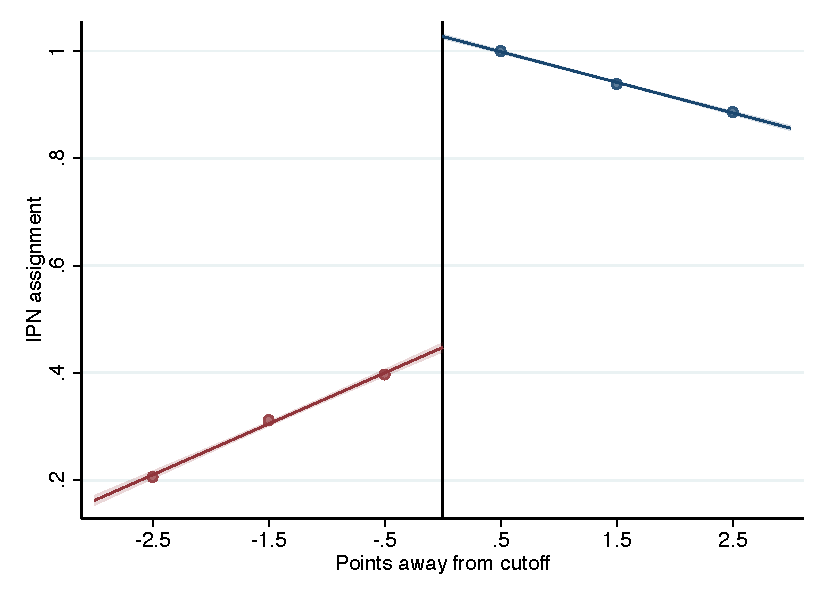
\includegraphics[width=\textwidth]{04_Figures/rd_plot_tau_IPN_assig_IPN3.pdf}
    \end{subfigure}}
\end{column}

\begin{column}{.5\textwidth}
\alt<2-5>{
    \begin{itemize}
        \item[]
        \item<3-> RD around the cutoff.
        \item<4-> Jump is not sharp since, student could be eligible at a lower-ranked school, and this school could also IPN.
        \item<5-> Still, we observe that \textcolor{blue}{treatment is higher to the right of the cutoff}.
    \end{itemize}}
    {\begin{subfigure}{\textwidth}
        \centering
        \caption{Assignment to an IPN HS around MID}
        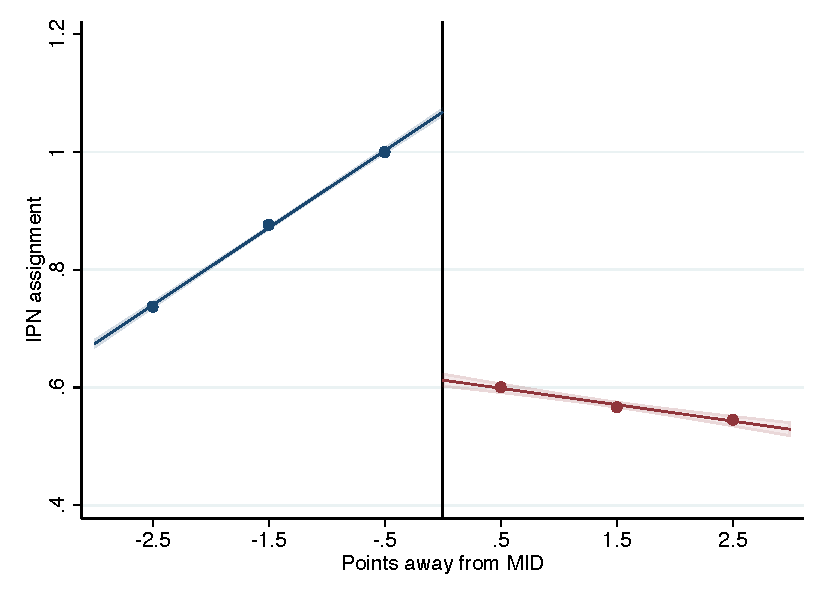
\includegraphics[width=\textwidth]{04_Figures/rd_plot_mid_IPN_assig_IPN3.pdf}
    \end{subfigure}}
\end{column}
\end{columns}

\label{fig:treat_rd_plot}    
\end{figure}}

\end{frame}

\subsection{Outcomes}

\begin{frame}[label=ITT_rd_plot_IPN,fragile]{RD plots of ITT effects for outcomes}
\hyperlink{ITT_rd_plot_IPN_app}{\beamergotobutton{ITT RD plots}}

\onslide<2-8>{
\begin{figure}
\begin{columns}[T]
\begin{column}{.5\textwidth}
\alt<5-7>{
    \begin{itemize}
        \item[]
        \item[]
        \item<6-> RD around the most informative disqualification (MID).
        \item<7-> Positive ITT effect of being marginally assigned to an IPN high school around the MID.
    \end{itemize}}
    {\begin{subfigure}{\textwidth}
        \centering
        \caption{Graduation rate around cutoff}
        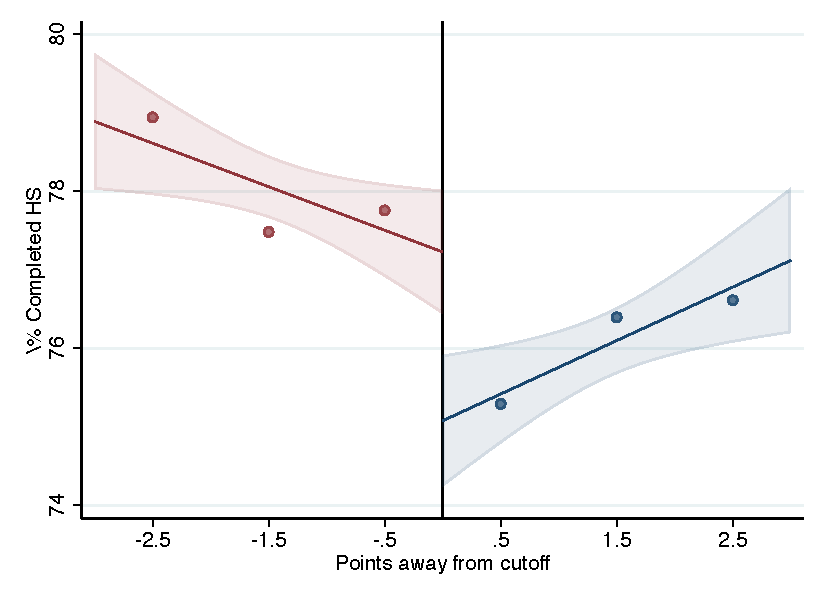
\includegraphics[width=\textwidth]{04_Figures/rd_plot_tau_bachillerato_mas_IPN3.pdf}
    \end{subfigure}}
\end{column}

\begin{column}{.5\textwidth}
\alt<2-4>{
    \begin{itemize}
        \item[]
        \item[]
        \item<3-> RD around the cutoff.
        \item<4-> Negative ITT effect of being marginally assigned to an IPN high school.
    \end{itemize}}
    {\begin{subfigure}{\textwidth}
        \centering
        \caption{Graduation rate around MID}
        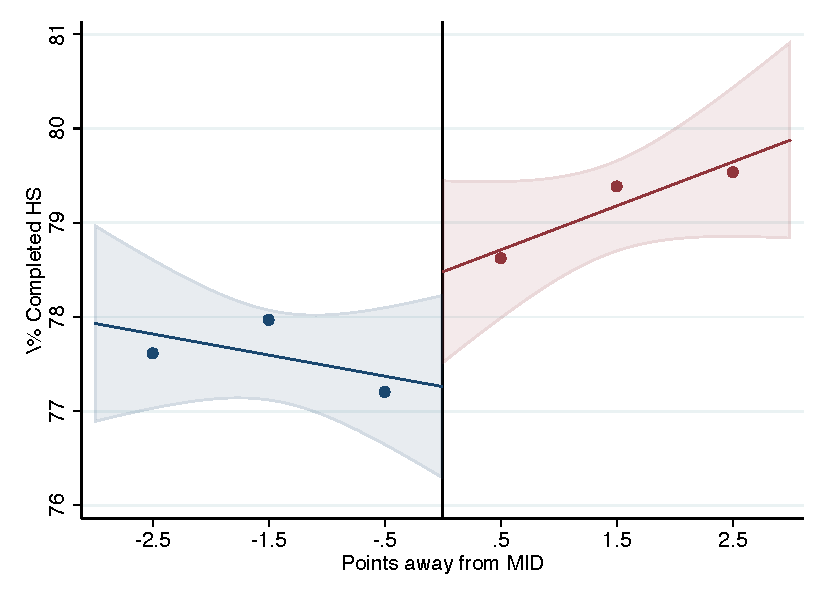
\includegraphics[width=\textwidth]{04_Figures/rd_plot_mid_bachillerato_mas_IPN3.pdf}
    \end{subfigure}}
\end{column}
\end{columns}

\label{fig:ITT_rd_plot_IPN}    
\end{figure}}

\end{frame}

\begin{frame}[fragile]{ITT effects of being assigned to an IPN HS}
\begin{table}[H]
\centering
\begin{adjustbox}{totalheight=0.88\textheight}
\begin{threeparttable}
\centering
%\caption{Intent to treat effects of being assigned to an IPN high-school}
\label{tab:ITT_Effect_INE_NoRun_IPN}
\begin{tabular}[t]{@{}l@{}l@{}l}
\toprule
\begin{tabular}[t]{lcc}
&	\multicolumn{2}{c}{1 point} \\
 \cmidrule(lr){2-3}
& Control &		Treatment 	\\ 
& mean & differential \\
&   (1) 	&  (2)		\\
\midrule
\% Voted (2018)     &       68.01&        0.18         \\
                    &     (46.65)&      (0.87)         \\
                    &     [6,206]&     [5,920]         \\
\% Crime (INE)      &        0.24&        0.00         \\
                    &      (4.91)&      (0.09)         \\
                    &     [6,206]&     [5,920]         \\
\% Death (INE)      &        0.37&        0.05         \\
                    &      (6.08)&      (0.12)         \\
                    &     [6,206]&     [5,920]         \\
\% INE expired      &        4.37&       -0.02         \\
                    &     (20.44)&      (0.37)         \\
                    &     [6,206]&     [5,920]         \\
\% Completed HS     &       79.39&       -4.47\sym{***}\\
                    &     (40.46)&      (0.80)         \\
                    &     [6,001]&     [5,734]         \\
\% Post-secondary education&       19.16&        0.19         \\
                    &     (39.36)&      (0.74)         \\
                    &     [6,001]&     [5,734]         \\
\% Unemployed       &        2.67&       -0.63\sym{**} \\
                    &     (16.11)&      (0.29)         \\
                    &     [6,001]&     [5,734]         \\
\% Housewife        &       10.01&        0.45         \\
                    &     (30.02)&      (0.92)         \\
                    &     [2,558]&     [2,436]         \\
\% Self-employed    &        3.27&       -0.18         \\
                    &     (17.78)&      (0.33)         \\
                    &     [6,001]&     [5,734]         \\

\end{tabular}
&
%\onslide<2->{
\begin{tabular}[t]{Hcc}
&	\multicolumn{2}{c}{2 points} \\
 \cmidrule(lr){2-3}
& Control &		Treatment 	\\ 
& mean & differential \\
&   (3) 	&  (4)		\\
\midrule
\% Voted (2012)     &       47.88&       -0.50         \\
                    &     (49.96)&      (0.60)         \\
                    &    [13,187]&    [11,215]         \\
\% Voted (2015)     &       34.62&        0.49         \\
                    &     (47.58)&      (0.64)         \\
                    &    [13,187]&    [11,215]         \\
\% Voted (2018)     &       67.51&        0.12         \\
                    &     (46.84)&      (0.62)         \\
                    &    [13,187]&    [11,215]         \\
\% Crime (INE)      &        0.28&       -0.04         \\
                    &      (5.29)&      (0.07)         \\
                    &    [13,187]&    [11,215]         \\
\% Death (INE)      &        0.43&       -0.11         \\
                    &      (6.56)&      (0.08)         \\
                    &    [13,187]&    [11,215]         \\
\% INE expired      &        4.46&       -0.28         \\
                    &     (20.64)&      (0.27)         \\
                    &    [13,187]&    [11,215]         \\
\% Completed HS     &       79.10&       -4.00\sym{***}\\
                    &     (40.66)&      (0.57)         \\
                    &    [12,737]&    [10,832]         \\
\% Post-secondary education&       18.99&        0.36         \\
                    &     (39.23)&      (0.53)         \\
                    &    [12,737]&    [10,832]         \\
\% Unemployed       &        2.83&       -0.47\sym{**} \\
                    &     (16.60)&      (0.22)         \\
                    &    [12,737]&    [10,832]         \\
\% Housewife        &        4.60&        0.13         \\
                    &     (20.95)&      (0.29)         \\
                    &    [12,737]&    [10,832]         \\
\% Self-employed    &        2.95&        0.24         \\
                    &     (16.93)&      (0.24)         \\
                    &    [12,737]&    [10,832]         \\

\end{tabular}
%}
&
%\onslide<3->{
\begin{tabular}[t]{Hcc}
&	\multicolumn{2}{c}{3 points} \\
 \cmidrule(lr){2-3}
& Control &		Treatment 	\\ 
& mean & differential \\
&   (5) 	&  (6)		\\
\midrule
\% Voted (2018)     &       67.23&       -0.14         \\
                    &     (46.94)&      (0.52)         \\
                    &    [20,255]&    [16,433]         \\
\% Crime (INE)      &        0.26&        0.01         \\
                    &      (5.11)&      (0.06)         \\
                    &    [20,255]&    [16,433]         \\
\% Death (INE)      &        0.38&        0.01         \\
                    &      (6.15)&      (0.07)         \\
                    &    [20,255]&    [16,433]         \\
\% INE expired      &        4.46&       -0.28         \\
                    &     (20.64)&      (0.22)         \\
                    &    [20,255]&    [16,433]         \\
\% Completed HS     &       79.43&       -4.32\sym{***}\\
                    &     (40.42)&      (0.47)         \\
                    &    [19,585]&    [15,881]         \\
\% Post-secondary education&       19.12&        0.12         \\
                    &     (39.32)&      (0.44)         \\
                    &    [19,585]&    [15,881]         \\
\% Unemployed       &        3.03&       -0.56\sym{***}\\
                    &     (17.15)&      (0.18)         \\
                    &    [19,585]&    [15,881]         \\
\% Housewife        &        4.57&        0.13         \\
                    &     (20.89)&      (0.24)         \\
                    &    [19,585]&    [15,881]         \\
\% Self-employed    &        2.86&        0.18         \\
                    &     (16.67)&      (0.19)         \\
                    &    [19,585]&    [15,881]         \\

\end{tabular}
%}
\tabularnewline \bottomrule
\end{tabular}
\end{threeparttable}
\end{adjustbox}
\end{table}
\end{frame}

\begin{frame}[fragile]{ITT effects of being assigned to an IPN HS using the cutoff}
\begin{table}[H]
\centering
\begin{adjustbox}{totalheight=0.88\textheight}
\begin{threeparttable}
\centering
%\caption{Intent to treat effects of being assigned to an IPN high-school}
\label{tab:ITT_Effect_INE_NoRun_IPN_tau}
\begin{tabular}[t]{@{}l@{}l@{}l}
\toprule
\begin{tabular}[t]{lcc}
&	\multicolumn{2}{c}{1 point} \\
 \cmidrule(lr){2-3}
& Control &		Treatment 	\\ 
& mean & differential \\
&   (1) 	&  (2)		\\
\midrule
\% Voted (2018)     &       66.78&        1.12         \\
                    &     (47.11)&      (1.06)         \\
                    &     [4,365]&     [4,287]         \\
\% Crime (INE)      &        0.25&        0.06         \\
                    &      (5.01)&      (0.12)         \\
                    &     [4,365]&     [4,287]         \\
\% Death (INE)      &        0.30&        0.10         \\
                    &      (5.45)&      (0.12)         \\
                    &     [4,365]&     [4,287]         \\
\% INE expired      &        4.49&        0.02         \\
                    &     (20.71)&      (0.45)         \\
                    &     [4,365]&     [4,287]         \\
\% Completed HS     &       78.90&       -5.48\sym{***}\\
                    &     (40.81)&      (0.97)         \\
                    &     [4,218]&     [4,147]         \\
\% Post-secondary education&       18.16&        0.34         \\
                    &     (38.56)&      (0.88)         \\
                    &     [4,218]&     [4,147]         \\
\% Unemployed       &        3.11&       -1.09\sym{***}\\
                    &     (17.35)&      (0.36)         \\
                    &     [4,218]&     [4,147]         \\
\% Housewife        &       11.73&       -0.49         \\
                    &     (32.19)&      (1.17)         \\
                    &     [1,722]&     [1,722]         \\
\% Self-employed    &        3.32&       -0.09         \\
                    &     (17.92)&      (0.41)         \\
                    &     [4,218]&     [4,147]         \\

\end{tabular}
&
%\onslide<2->{
\begin{tabular}[t]{Hcc}
&	\multicolumn{2}{c}{2 points} \\
 \cmidrule(lr){2-3}
& Control &		Treatment 	\\ 
& mean & differential \\
&   (3) 	&  (4)		\\
\midrule
\% Voted (2012)     &       47.10&       -0.36         \\
                    &     (49.92)&      (0.69)         \\
                    &     [9,790]&     [8,852]         \\
\% Voted (2015)     &       33.85&        0.75         \\
                    &     (47.32)&      (0.73)         \\
                    &     [9,790]&     [8,852]         \\
\% Voted (2018)     &       66.47&        0.49         \\
                    &     (47.21)&      (0.73)         \\
                    &     [9,790]&     [8,852]         \\
\% Crime (INE)      &        0.31&        0.02         \\
                    &      (5.53)&      (0.09)         \\
                    &     [9,790]&     [8,852]         \\
\% Death (INE)      &        0.41&       -0.07         \\
                    &      (6.38)&      (0.09)         \\
                    &     [9,790]&     [8,852]         \\
\% INE expired      &        4.69&       -0.23         \\
                    &     (21.14)&      (0.31)         \\
                    &     [9,790]&     [8,852]         \\
\% Completed HS     &       78.46&       -4.51\sym{***}\\
                    &     (41.11)&      (0.67)         \\
                    &     [9,451]&     [8,541]         \\
\% Post-secondary education&       18.33&        0.47         \\
                    &     (38.69)&      (0.60)         \\
                    &     [9,451]&     [8,541]         \\
\% Unemployed       &        3.26&       -0.76\sym{***}\\
                    &     (17.76)&      (0.27)         \\
                    &     [9,451]&     [8,541]         \\
\% Housewife        &        5.14&       -0.19         \\
                    &     (22.09)&      (0.35)         \\
                    &     [9,451]&     [8,541]         \\
\% Self-employed    &        3.04&        0.27         \\
                    &     (17.16)&      (0.28)         \\
                    &     [9,451]&     [8,541]         \\

\end{tabular}
%}
&
%\onslide<3->{
\begin{tabular}[t]{Hcc}
&	\multicolumn{2}{c}{3 points} \\
 \cmidrule(lr){2-3}
& Control &		Treatment 	\\ 
& mean & differential \\
&   (5) 	&  (6)		\\
\midrule
\% Voted (2012)     &       47.32&       -0.13         \\
                    &     (49.93)&      (0.56)         \\
                    &    [15,605]&    [13,764]         \\
\% Voted (2015)     &       33.88&        0.61         \\
                    &     (47.33)&      (0.60)         \\
                    &    [15,605]&    [13,764]         \\
\% Voted (2018)     &       66.20&        0.14         \\
                    &     (47.30)&      (0.59)         \\
                    &    [15,605]&    [13,764]         \\
\% Crime (INE)      &        0.28&        0.06         \\
                    &      (5.24)&      (0.07)         \\
                    &    [15,605]&    [13,764]         \\
\% Death (INE)      &        0.35&        0.06         \\
                    &      (5.93)&      (0.08)         \\
                    &    [15,605]&    [13,764]         \\
\% INE expired      &        4.72&       -0.39         \\
                    &     (21.20)&      (0.25)         \\
                    &    [15,605]&    [13,764]         \\
\% Completed HS     &       78.65&       -4.41\sym{***}\\
                    &     (40.98)&      (0.54)         \\
                    &    [15,075]&    [13,301]         \\
\% Post-secondary education&       18.16&        0.62         \\
                    &     (38.55)&      (0.49)         \\
                    &    [15,075]&    [13,301]         \\
\% Unemployed       &        3.43&       -0.89\sym{***}\\
                    &     (18.20)&      (0.21)         \\
                    &    [15,075]&    [13,301]         \\
\% Housewife        &        5.02&       -0.02         \\
                    &     (21.84)&      (0.28)         \\
                    &    [15,075]&    [13,301]         \\
\% Self-employed    &        2.97&        0.22         \\
                    &     (16.98)&      (0.22)         \\
                    &    [15,075]&    [13,301]         \\

\end{tabular}
%}
\tabularnewline \bottomrule
\end{tabular}
\end{threeparttable}
\end{adjustbox}
\end{table}
\end{frame}

\begin{frame}[fragile]{ITT effects of being assigned to an IPN HS using the MID}
\begin{table}[H]
\centering
\begin{adjustbox}{totalheight=0.88\textheight}
\begin{threeparttable}
\centering
%\caption{Intent to treat effects of being assigned to an IPN high-school}
\label{tab:ITT_Effect_INE_NoRun_IPN_mid}
\begin{tabular}[t]{@{}l@{}l@{}l}
\toprule
\begin{tabular}[t]{lcc}
&	\multicolumn{2}{c}{1 point} \\
 \cmidrule(lr){2-3}
& Control &		Treatment 	\\ 
& mean & differential \\
&   (1) 	&  (2)		\\
\midrule
\% Voted (2018)     &       70.83&       -1.74         \\
                    &     (45.47)&      (1.74)         \\
                    &     [1,563]&     [1,699]         \\
\% Crime (INE)      &        0.19&       -0.14         \\
                    &      (4.38)&      (0.13)         \\
                    &     [1,563]&     [1,699]         \\
\% Death (INE)      &        0.51&        0.00         \\
                    &      (7.14)&      (0.28)         \\
                    &     [1,563]&     [1,699]         \\
\% INE expired      &        3.90&        0.31         \\
                    &     (19.37)&      (0.71)         \\
                    &     [1,563]&     [1,699]         \\
\% Completed HS     &       80.62&       -1.68         \\
                    &     (39.54)&      (1.57)         \\
                    &     [1,512]&     [1,649]         \\
\% Post-secondary education&       21.69&       -0.49         \\
                    &     (41.23)&      (1.57)         \\
                    &     [1,512]&     [1,649]         \\
\% Unemployed       &        1.59&        0.25         \\
                    &     (12.50)&      (0.48)         \\
                    &     [1,512]&     [1,649]         \\
\% Housewife        &        2.58&        1.54\sym{**} \\
                    &     (15.86)&      (0.67)         \\
                    &     [1,512]&     [1,649]         \\
\% Self-employed    &        2.65&        0.05         \\
                    &     (16.05)&      (0.62)         \\
                    &     [1,512]&     [1,649]         \\

\end{tabular}
&
%\onslide<2->{
\begin{tabular}[t]{Hcc}
&	\multicolumn{2}{c}{2 points} \\
 \cmidrule(lr){2-3}
& Control &		Treatment 	\\ 
& mean & differential \\
&   (3) 	&  (4)		\\
\midrule
\% Voted (2018)     &       71.06&        0.14         \\
                    &     (45.36)&      (1.13)         \\
                    &     [3,880]&     [4,051]         \\
\% Crime (INE)      &        0.26&       -0.24\sym{***}\\
                    &      (5.07)&      (0.09)         \\
                    &     [3,880]&     [4,051]         \\
\% Death (INE)      &        0.39&       -0.09         \\
                    &      (6.21)&      (0.15)         \\
                    &     [3,880]&     [4,051]         \\
\% INE expired      &        3.38&       -0.07         \\
                    &     (18.06)&      (0.43)         \\
                    &     [3,880]&     [4,051]         \\
\% Completed HS     &       80.81&       -2.53\sym{**} \\
                    &     (39.38)&      (1.03)         \\
                    &     [3,742]&     [3,907]         \\
\% Post-secondary education&       20.34&        0.38         \\
                    &     (40.26)&      (1.00)         \\
                    &     [3,742]&     [3,907]         \\
\% Unemployed       &        1.71&        0.20         \\
                    &     (12.97)&      (0.33)         \\
                    &     [3,742]&     [3,907]         \\
\% Housewife        &        3.05&        1.34\sym{***}\\
                    &     (17.19)&      (0.46)         \\
                    &     [3,742]&     [3,907]         \\
\% Self-employed    &        2.67&        0.04         \\
                    &     (16.13)&      (0.41)         \\
                    &     [3,742]&     [3,907]         \\

\end{tabular}
%}
&
%\onslide<3->{
\begin{tabular}[t]{Hcc}
&	\multicolumn{2}{c}{3 points} \\
 \cmidrule(lr){2-3}
& Control &		Treatment 	\\ 
& mean & differential \\
&   (5) 	&  (6)		\\
\midrule
\% Voted (2018)     &       70.70&       -0.23         \\
                    &     (45.52)&      (0.87)         \\
                    &     [6,816]&     [7,474]         \\
\% Crime (INE)      &        0.19&       -0.07         \\
                    &      (4.36)&      (0.06)         \\
                    &     [6,816]&     [7,474]         \\
\% Death (INE)      &        0.40&       -0.03         \\
                    &      (6.28)&      (0.12)         \\
                    &     [6,816]&     [7,474]         \\
\% INE expired      &        3.45&       -0.23         \\
                    &     (18.25)&      (0.33)         \\
                    &     [6,816]&     [7,474]         \\
\% Completed HS     &       80.95&       -3.86\sym{***}\\
                    &     (39.27)&      (0.78)         \\
                    &     [6,619]&     [7,240]         \\
\% Post-secondary education&       20.71&       -0.40         \\
                    &     (40.53)&      (0.76)         \\
                    &     [6,619]&     [7,240]         \\
\% Unemployed       &        1.84&        0.33         \\
                    &     (13.45)&      (0.27)         \\
                    &     [6,619]&     [7,240]         \\
\% Housewife        &        6.51&        1.53\sym{**} \\
                    &     (24.68)&      (0.76)         \\
                    &     [2,902]&     [3,136]         \\
\% Self-employed    &        2.57&        0.06         \\
                    &     (15.82)&      (0.32)         \\
                    &     [6,619]&     [7,240]         \\

\end{tabular}
%}
\tabularnewline \bottomrule
\end{tabular}
\end{threeparttable}
\end{adjustbox}
\end{table}
\end{frame}

\section{Conclusions}
\begin{frame}[plain]{What can we take away from this?}
\begin{itemize}
\vfill \item Treatment effect heterogeneity matters a lot
\vfill \item Still lots to do
\vfill \item We aim to 
\begin{enumerate}
\vfill \item Estimate the marginal treatment effect distribution at each school exploiting the ``cutoffs'' for the next best option of each applicant \tiny{\citep{NBERw22363,Kowalski2021,Kowalski}}

\vfill \item \normalsize Estimate ``value added'' of different schools on different outcomes, for different children

\vfill \item How do these VA estimates correlate, and what drives parental demand \tiny{\citep{Kirabo2020,Beuermann2022}}
\end{enumerate}
\end{itemize}
\end{frame}

\begin{frame}[plain]{Thank you}
\begin{itemize}
 \item Questions? Thoughts? Comments?
\vfill \item Please reach out: \href{mailto:mtromero@itam.mx}{mtromero@itam.mx}
\end{itemize}
\end{frame}


\section{References}
\begin{frame}[allowframebreaks]{References}
\bibliographystyle{ecta}
\bibliography{05_Report/01_Paper/References}
\end{frame}

\section{Appendix}
\begin{transitionframe}
  \begin{center}
    \Huge \textcolor{white}{Appendix}
  \end{center}
\end{transitionframe}

\appendix

\subsection{Balance RD Plots}

\begin{transitionframe}
  \begin{center}
    \Huge \textcolor{white}{Balance RD Plots}
  \end{center}
\end{transitionframe}

\begin{frame}[label=balance_rd_plot_app]{RD plots for balance variables}
\hyperlink{balance_rd_plot}{\beamergotobutton{Back}}
\begin{figure}

    \begin{subfigure}{0.45\textwidth}
        \centering
        \caption{Age (2018) around cutoff}
        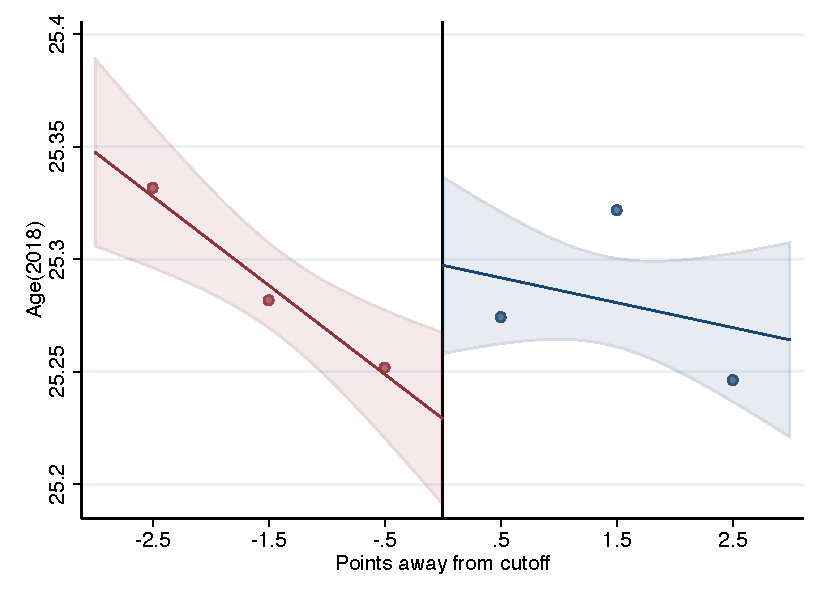
\includegraphics[width=\textwidth]{04_Figures/rd_plot_tau_age2018_IPN3.pdf}
    \end{subfigure}
    \begin{subfigure}{0.45\textwidth}
        \centering
        \caption{Age (2018) plot around MID}
        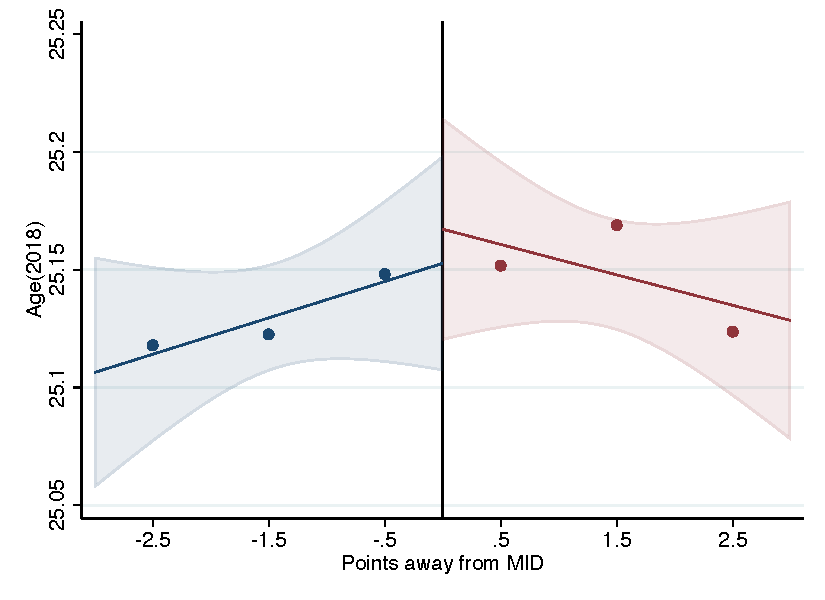
\includegraphics[width=\textwidth]{04_Figures/rd_plot_mid_age2018_IPN3.pdf}
    \end{subfigure}
    
\end{figure}
\end{frame}

\begin{frame}{RD plots for balance variables}
\hyperlink{balance_rd_plot}{\beamergotobutton{Back}}
\begin{figure}

    \begin{subfigure}{0.45\textwidth}
        \centering
        \caption{Male around cutoff}
        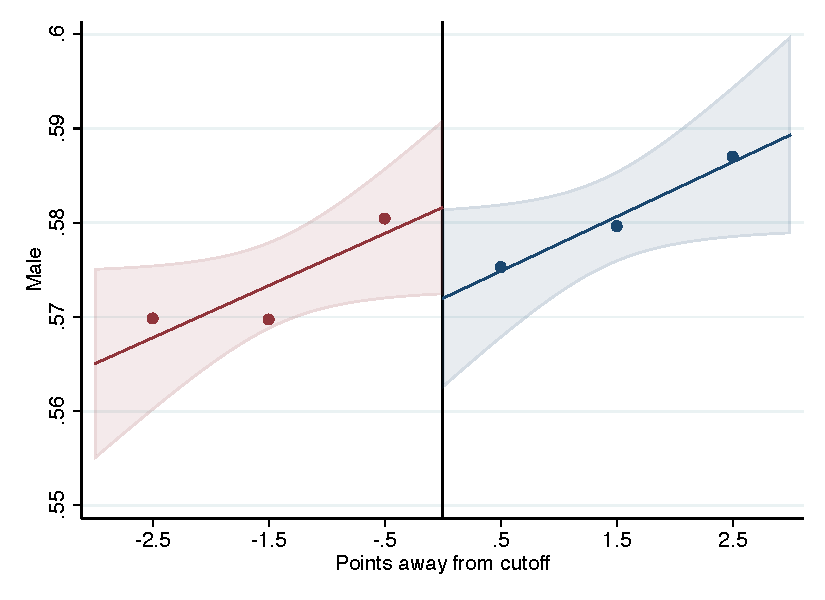
\includegraphics[width=\textwidth]{04_Figures/rd_plot_tau_hombre_IPN3.pdf}
    \end{subfigure}
    \begin{subfigure}{0.45\textwidth}
        \centering
        \caption{Male around MID}
        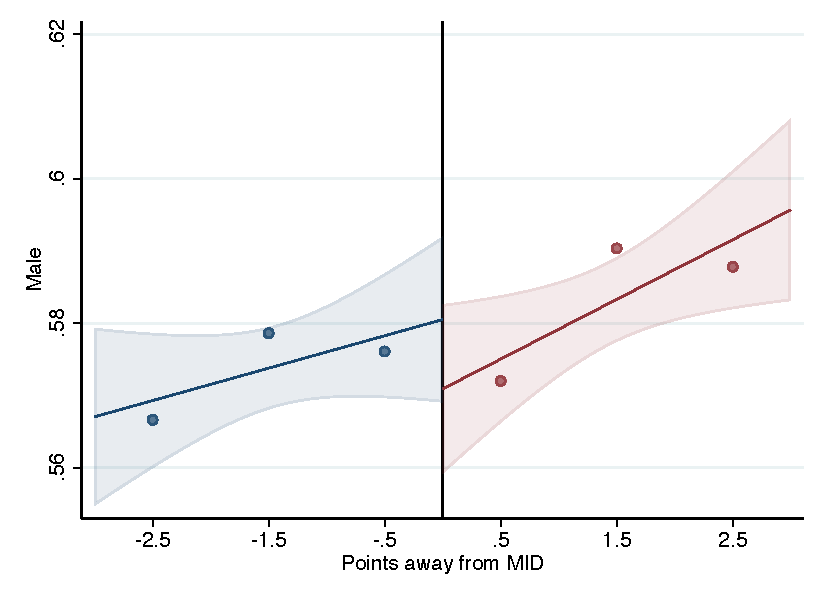
\includegraphics[width=\textwidth]{04_Figures/rd_plot_mid_hombre_IPN3.pdf}
    \end{subfigure}
    
\end{figure}
\end{frame}

\begin{frame}{RD plots for balance variables}
\hyperlink{balance_rd_plot}{\beamergotobutton{Back}}
\begin{figure}

    \begin{subfigure}{0.45\textwidth}
        \centering
        \caption{Private (middle school) around cutoff}
        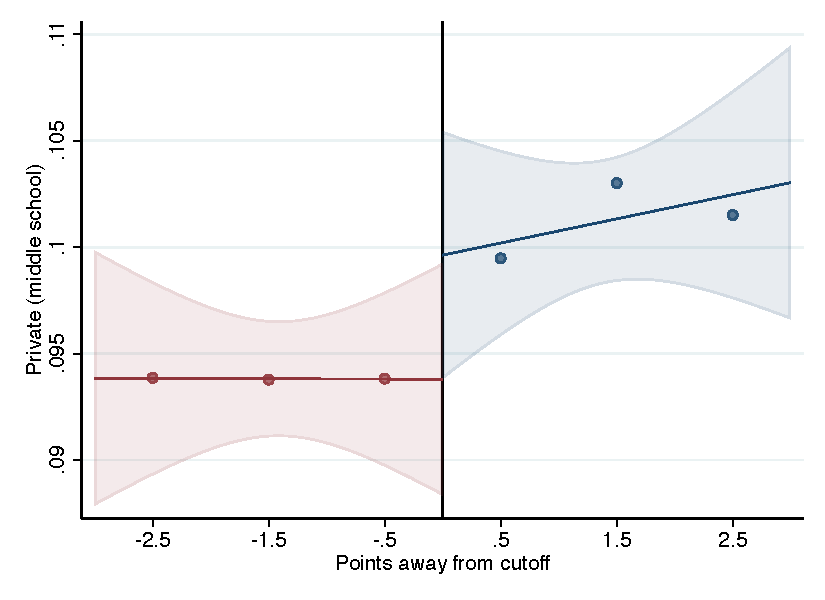
\includegraphics[width=\textwidth]{04_Figures/rd_plot_tau_Secundaria_Privada_IPN3.pdf}
    \end{subfigure}
    \begin{subfigure}{0.45\textwidth}
        \centering
        \caption{Private (middle school) around MID}
        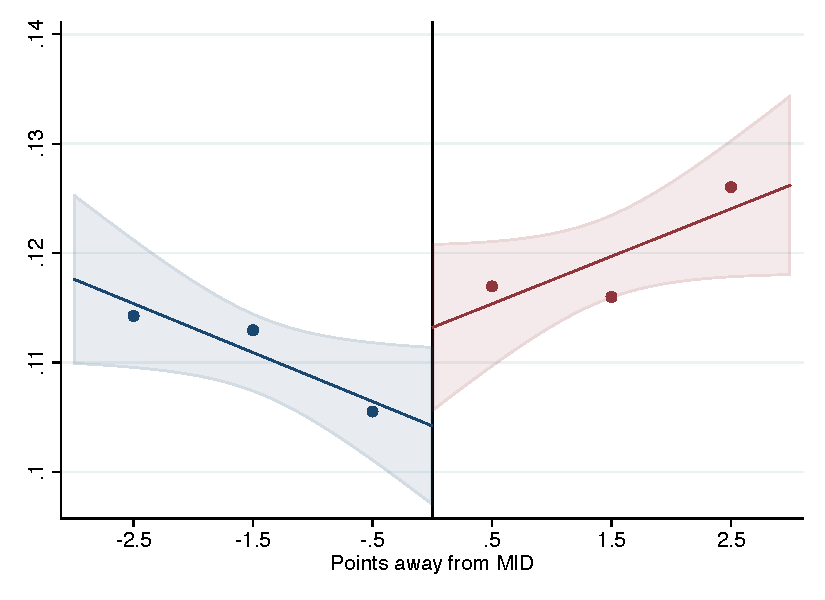
\includegraphics[width=\textwidth]{04_Figures/rd_plot_mid_Secundaria_Privada_IPN3.pdf}
    \end{subfigure}
    
\end{figure}
\end{frame}

\begin{frame}{RD plots for balance variables}
\hyperlink{balance_rd_plot}{\beamergotobutton{Back}}
\begin{figure}

    \begin{subfigure}{0.45\textwidth}
        \centering
        \caption{GPA (middle school) around cutoff}
        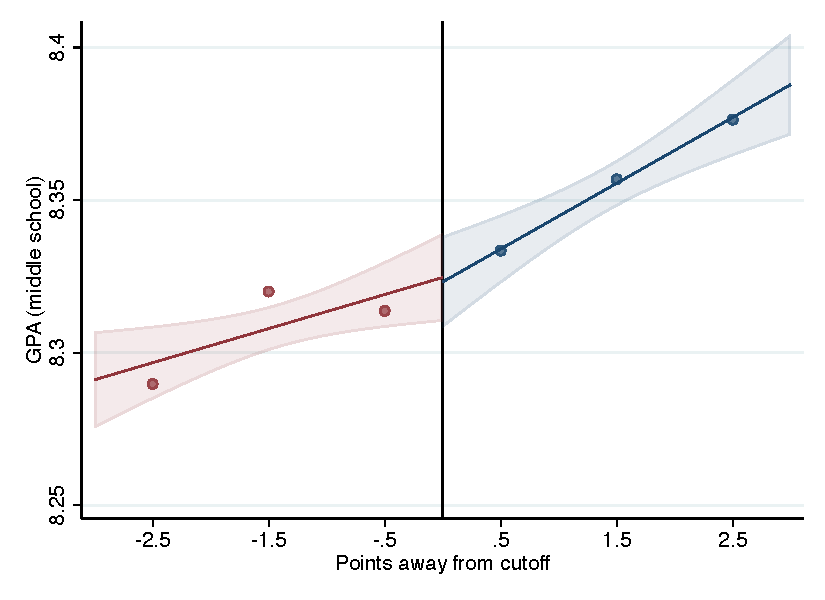
\includegraphics[width=\textwidth]{04_Figures/rd_plot_tau_sus_prom_IPN3.pdf}
    \end{subfigure}
    \begin{subfigure}{0.45\textwidth}
        \centering
        \caption{GPA (middle school) around MID}
        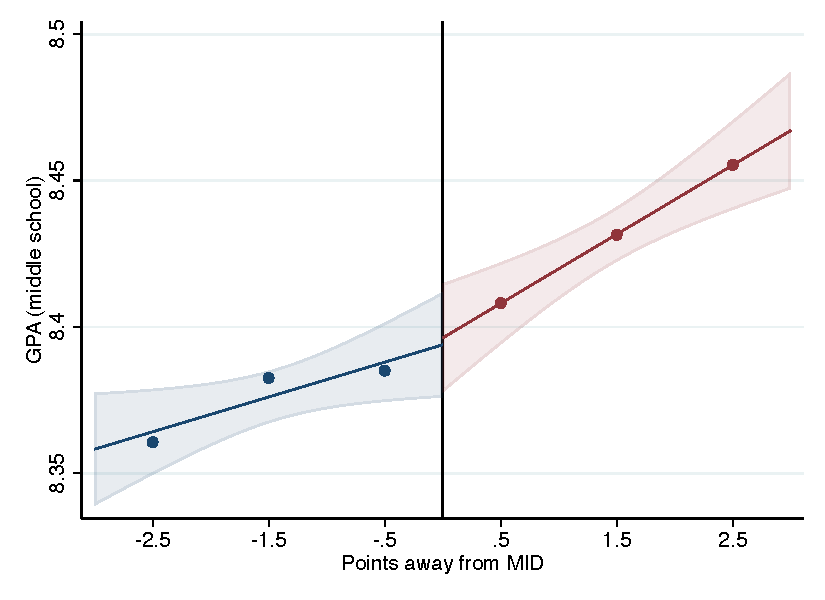
\includegraphics[width=\textwidth]{04_Figures/rd_plot_mid_sus_prom_IPN3.pdf}
    \end{subfigure}
    
\end{figure}
\end{frame}

\begin{frame}{RD plots for balance variables}
\hyperlink{balance_rd_plot}{\beamergotobutton{Back}}
\begin{figure}

    \begin{subfigure}{0.45\textwidth}
        \centering
        \caption{Middle school graduation around cutoff}
        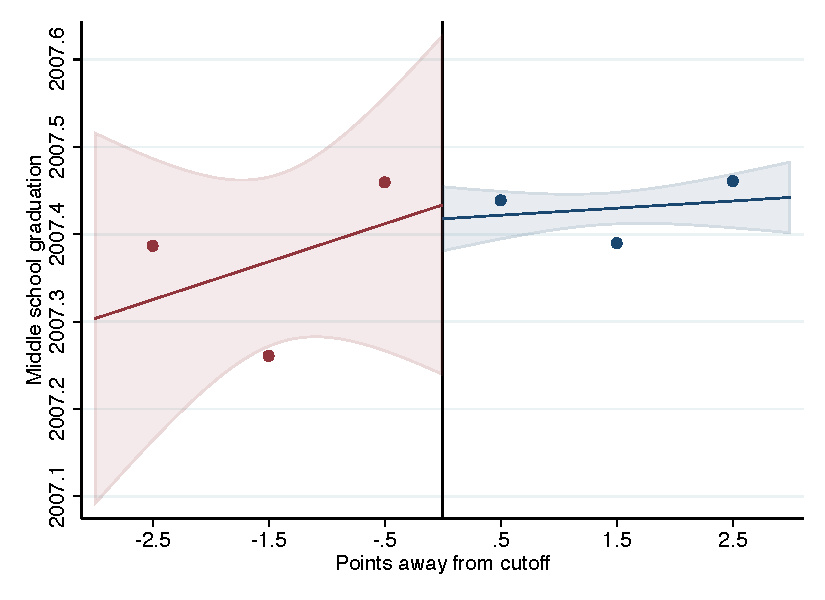
\includegraphics[width=\textwidth]{04_Figures/rd_plot_tau_ano_cert_IPN3.pdf}
    \end{subfigure}
    \begin{subfigure}{0.45\textwidth}
        \centering
        \caption{Middle school graduation around MID}
        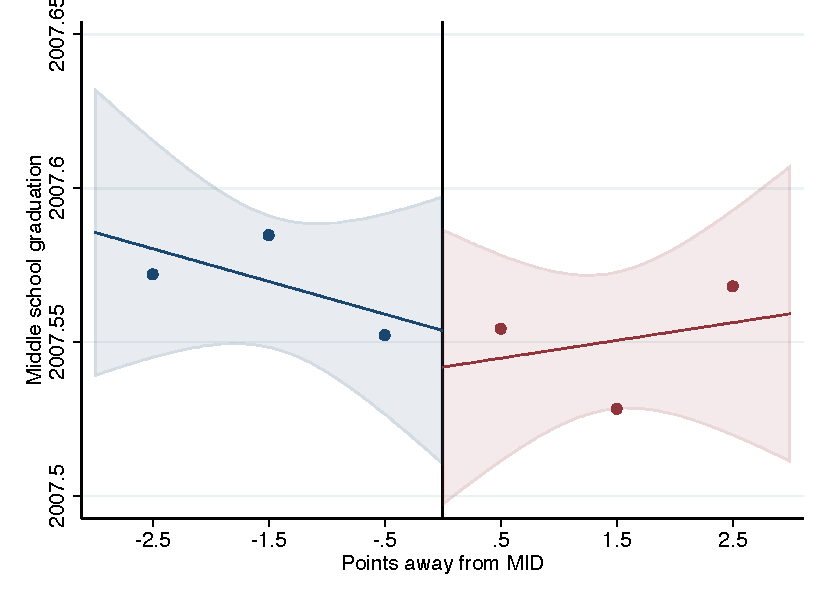
\includegraphics[width=\textwidth]{04_Figures/rd_plot_mid_ano_cert_IPN3.pdf}
    \end{subfigure}
    
\end{figure}
\end{frame}

\begin{frame}{RD plots for balance variables}
\hyperlink{balance_rd_plot}{\beamergotobutton{Back}}
\begin{figure}

    \begin{subfigure}{0.45\textwidth}
        \centering
        \caption{Father's age around cutoff}
        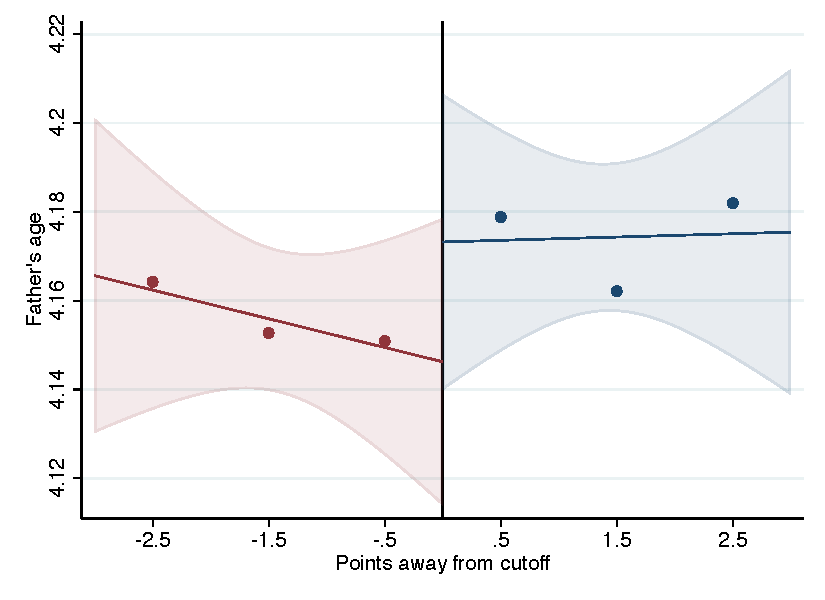
\includegraphics[width=\textwidth]{04_Figures/rd_plot_tau_edad_pad_IPN3.pdf}
    \end{subfigure}
    \begin{subfigure}{0.45\textwidth}
        \centering
        \caption{Father's age graduation around MID}
        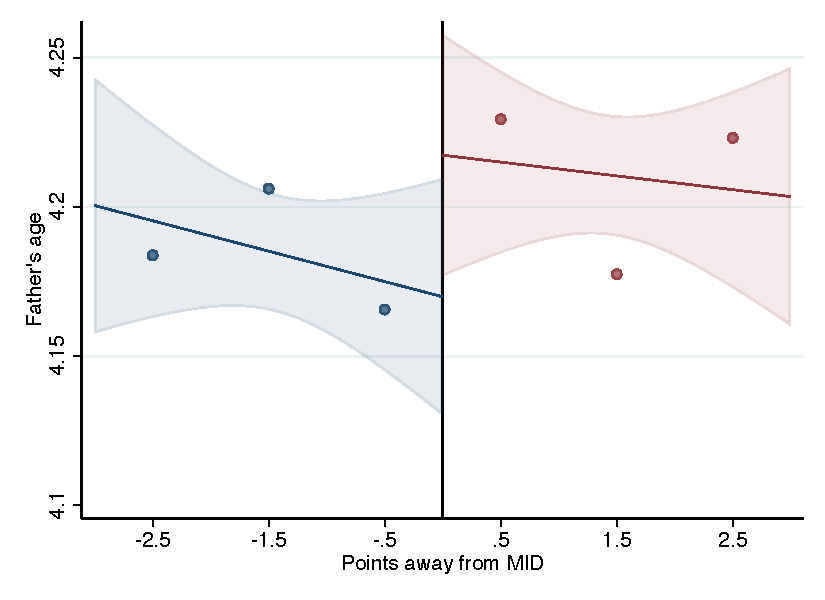
\includegraphics[width=\textwidth]{04_Figures/rd_plot_mid_edad_pad_IPN3.pdf}
    \end{subfigure}
    
\end{figure}
\end{frame}

\begin{frame}{RD plots for balance variables}
\hyperlink{balance_rd_plot}{\beamergotobutton{Back}}
\begin{figure}

    \begin{subfigure}{0.45\textwidth}
        \centering
        \caption{Mother's age around cutoff}
        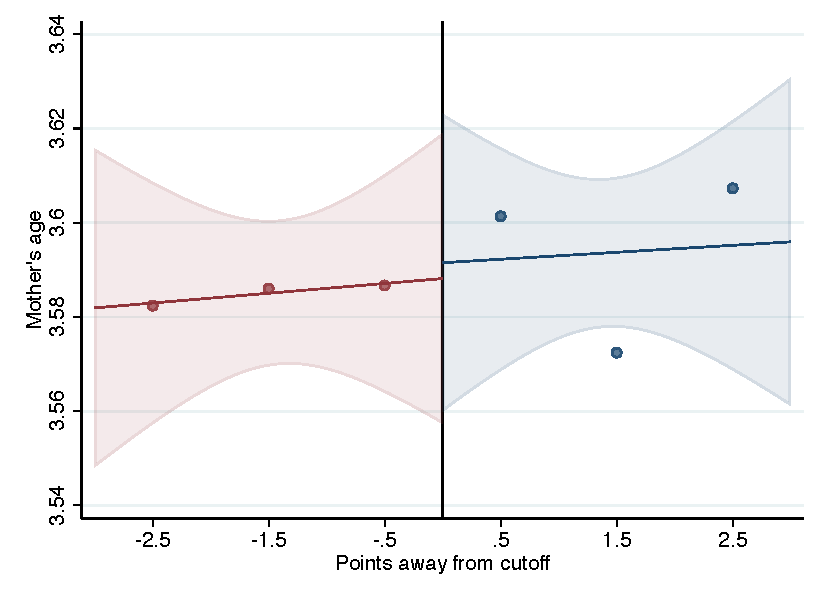
\includegraphics[width=\textwidth]{04_Figures/rd_plot_tau_edad_mad_IPN3.pdf}
    \end{subfigure}
    \begin{subfigure}{0.45\textwidth}
        \centering
        \caption{Mother's age graduation around MID}
        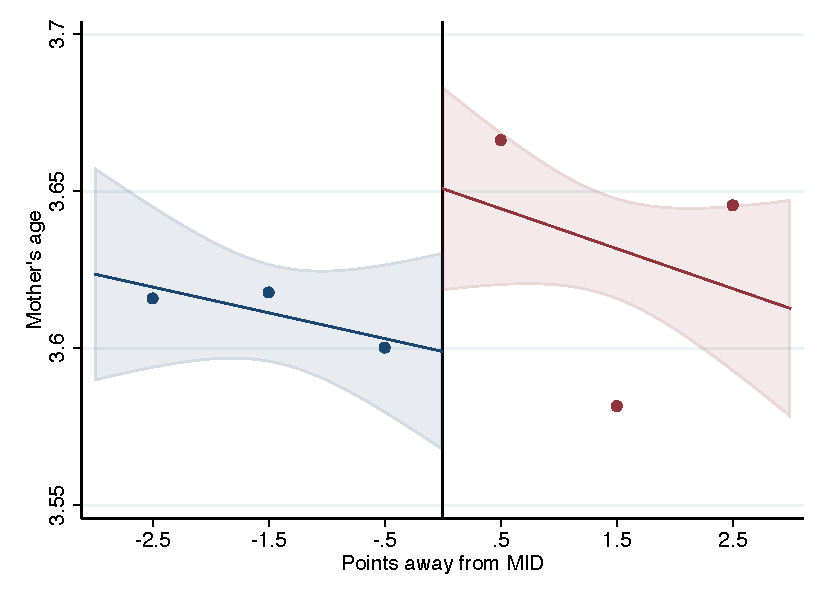
\includegraphics[width=\textwidth]{04_Figures/rd_plot_mid_edad_mad_IPN3.pdf}
    \end{subfigure}
    
\end{figure}
\end{frame}

\subsection{ITT RD Plots}

\begin{transitionframe}
  \begin{center}
    \Huge \textcolor{white}{ITT RD Plots}
  \end{center}
\end{transitionframe}

\begin{frame}[label=ITT_rd_plot_IPN_app]{RD plots of ITT effects for outcomes}
\hyperlink{ITT_rd_plot_IPN}{\beamergotobutton{Back}}
\begin{figure}

    \begin{subfigure}{0.45\textwidth}
        \centering
        \caption{Graduated (\%) around cutoff}
        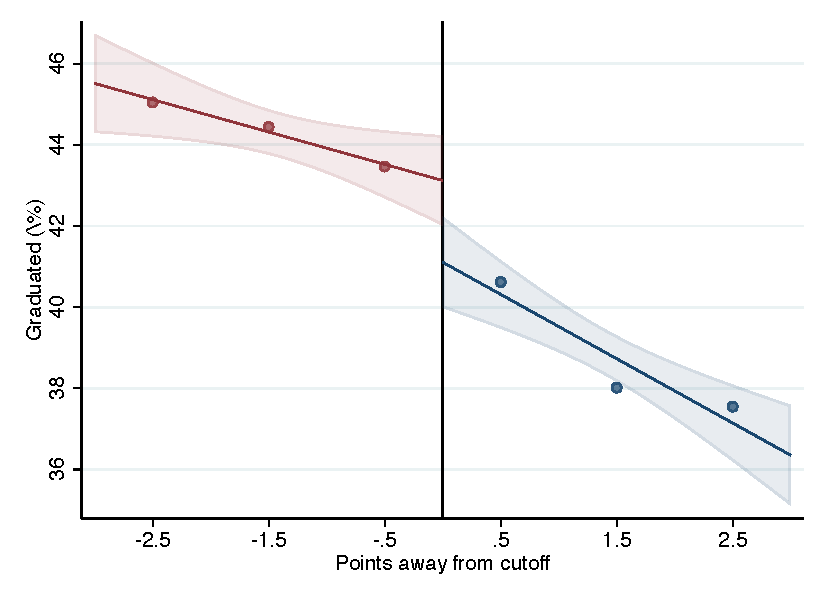
\includegraphics[width=\textwidth]{04_Figures/rd_plot_tau_ENLACE_ANY_IPN3.pdf}
    \end{subfigure}
    \begin{subfigure}{0.45\textwidth}
        \centering
        \caption{Graduated (\%) around MID}
        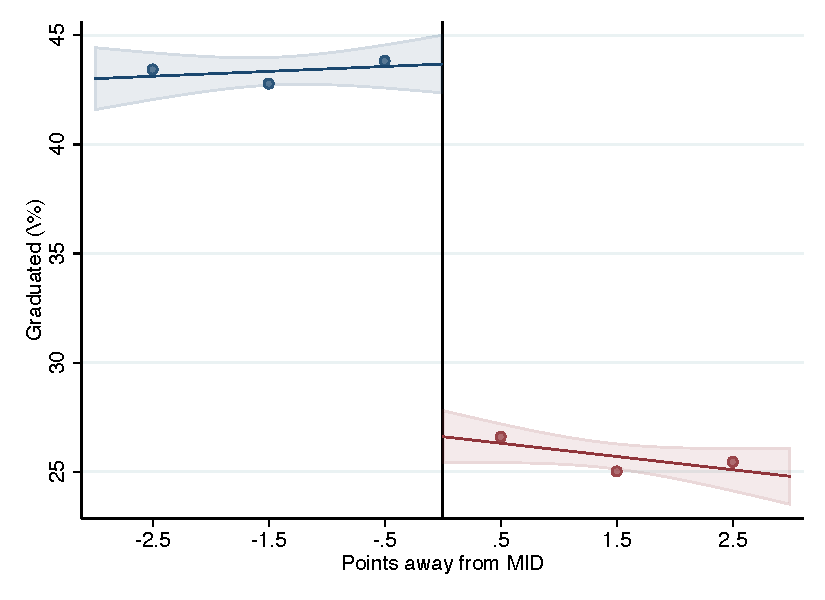
\includegraphics[width=\textwidth]{04_Figures/rd_plot_mid_ENLACE_ANY_IPN3.pdf}
    \end{subfigure}
    
\end{figure}
\end{frame}

\begin{frame}{RD plots of ITT effects for outcomes}
\hyperlink{ITT_rd_plot_IPN}{\beamergotobutton{Back}}
\begin{figure}

    \begin{subfigure}{0.45\textwidth}
        \centering
        \caption{Graduated from private (\%) around cutoff}
        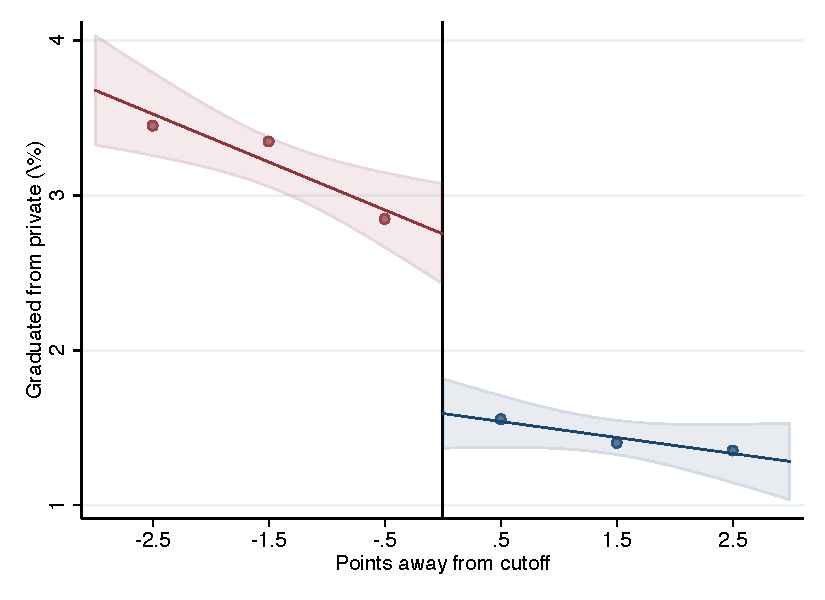
\includegraphics[width=\textwidth]{04_Figures/rd_plot_tau_ENLACE_Privado_Un_IPN3.pdf}
    \end{subfigure}
    \begin{subfigure}{0.45\textwidth}
        \centering
        \caption{Graduated from private (\%) around MID}
        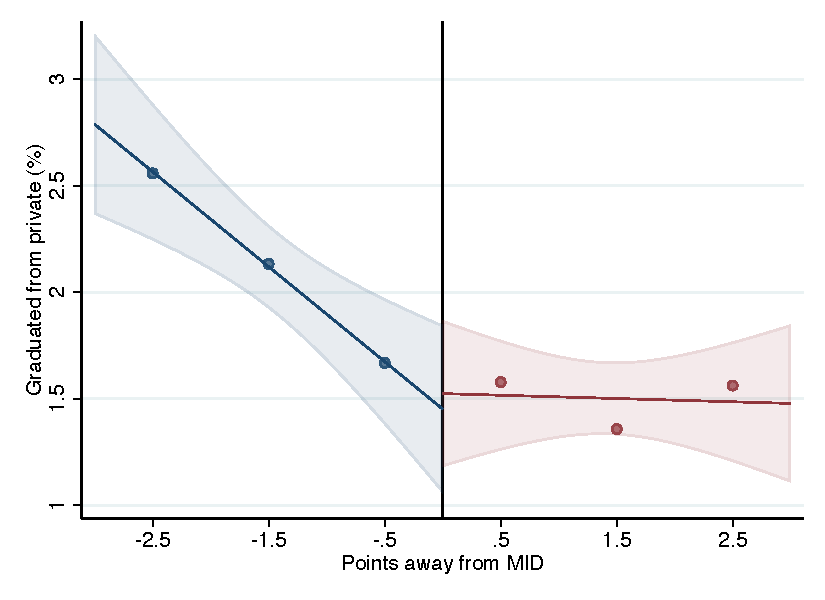
\includegraphics[width=\textwidth]{04_Figures/rd_plot_mid_ENLACE_Privado_Un_IPN3.pdf}
    \end{subfigure}
    
\end{figure}
\end{frame}

\begin{frame}{RD plots of ITT effects for outcomes}
\hyperlink{ITT_rd_plot_IPN}{\beamergotobutton{Back}}
\begin{figure}

    \begin{subfigure}{0.45\textwidth}
        \centering
        \caption{Graduated from private (\%) | Grad around cutoff}
        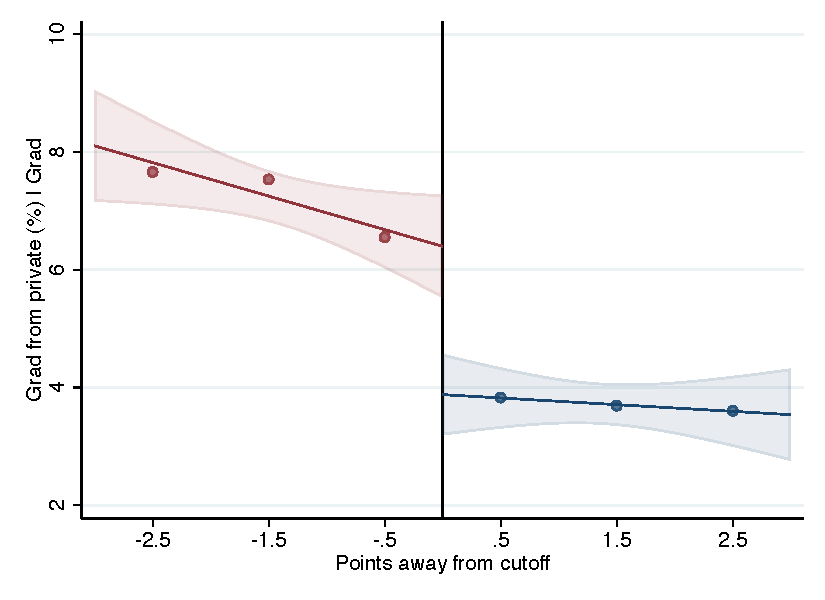
\includegraphics[width=\textwidth]{04_Figures/rd_plot_tau_ENLACE_Privado_IPN3.pdf}
    \end{subfigure}
    \begin{subfigure}{0.45\textwidth}
        \centering
        \caption{Graduated from private (\%) | Grad around MID}
        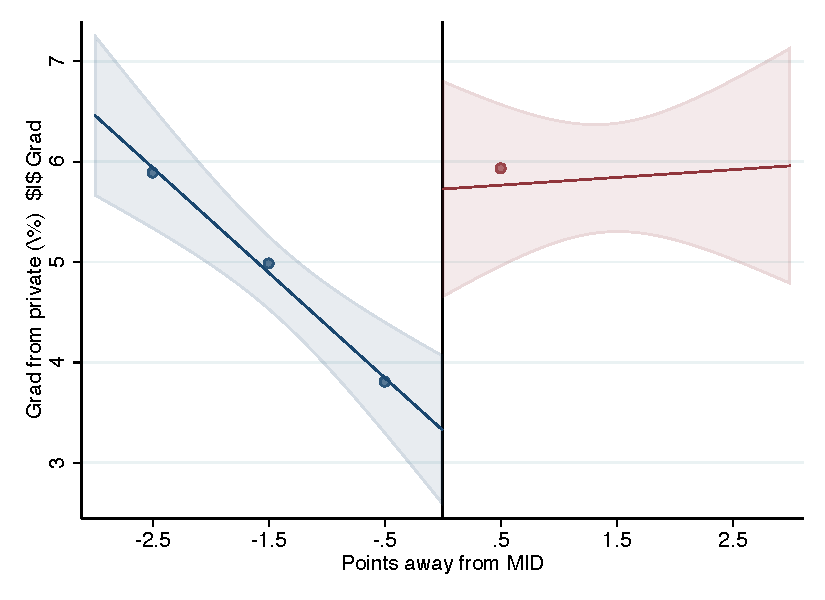
\includegraphics[width=\textwidth]{04_Figures/rd_plot_mid_ENLACE_Privado_IPN3.pdf}
    \end{subfigure}
    
\end{figure}
\end{frame}

\begin{frame}{RD plots of ITT effects for outcomes}
\hyperlink{ITT_rd_plot_IPN}{\beamergotobutton{Back}}
\begin{figure}

    \begin{subfigure}{0.45\textwidth}
        \centering
        \caption{Spanish (ENLACE | Grad) around cutoff}
        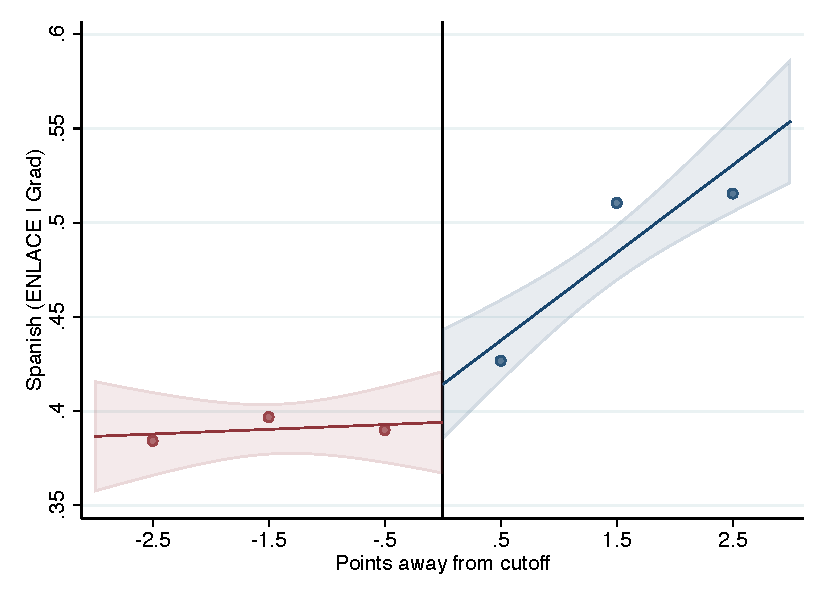
\includegraphics[width=\textwidth]{04_Figures/rd_plot_tau_p_esp_3_IPN3.pdf}
    \end{subfigure}
    \begin{subfigure}{0.45\textwidth}
        \centering
        \caption{Spanish (ENLACE | Grad) around MID}
        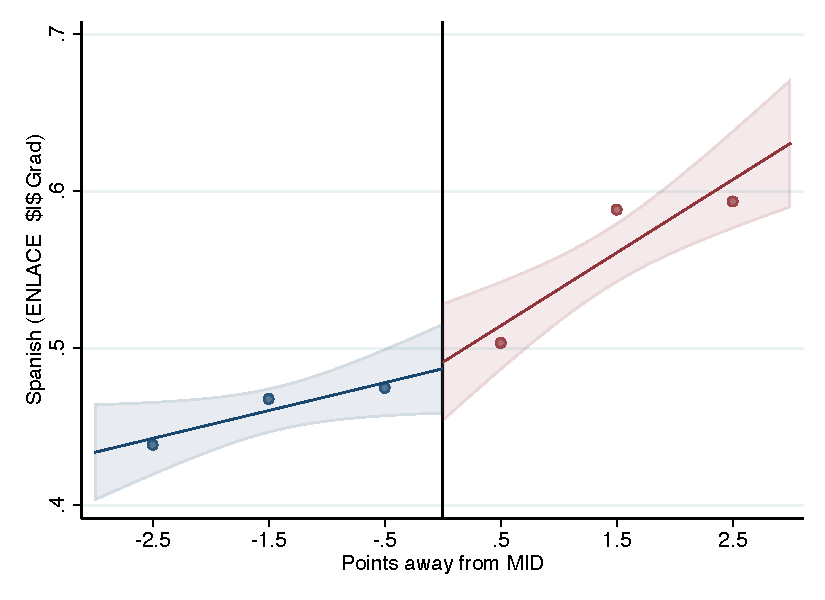
\includegraphics[width=\textwidth]{04_Figures/rd_plot_mid_p_esp_3_IPN3.pdf}
    \end{subfigure}
    
\end{figure}
\end{frame}

\begin{frame}{RD plots of ITT effects for outcomes}
\hyperlink{ITT_rd_plot_IPN}{\beamergotobutton{Back}}
\begin{figure}

    \begin{subfigure}{0.45\textwidth}
        \centering
        \caption{Math (ENLACE | Grad) around cutoff}
        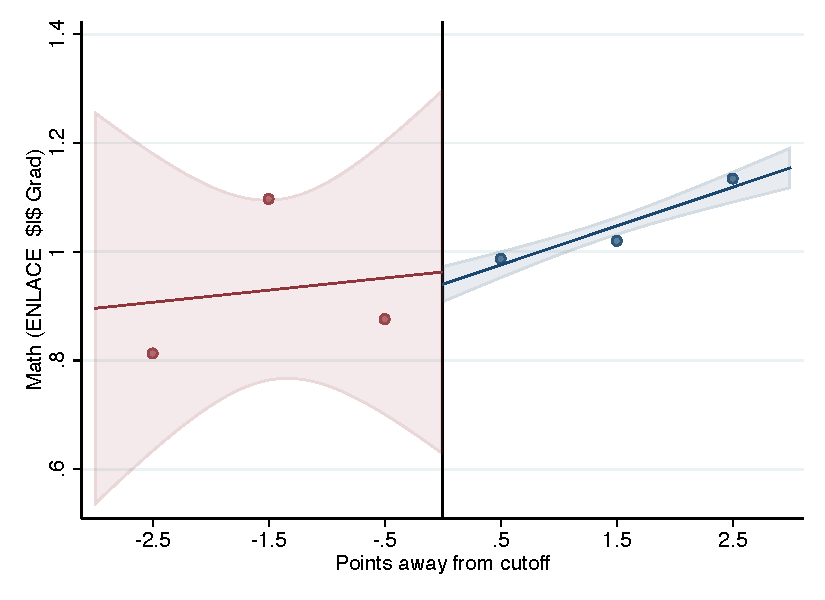
\includegraphics[width=\textwidth]{04_Figures/rd_plot_tau_p_mat_3_IPN3.pdf}
    \end{subfigure}
    \begin{subfigure}{0.45\textwidth}
        \centering
        \caption{Math (ENLACE | Grad) around MID}
        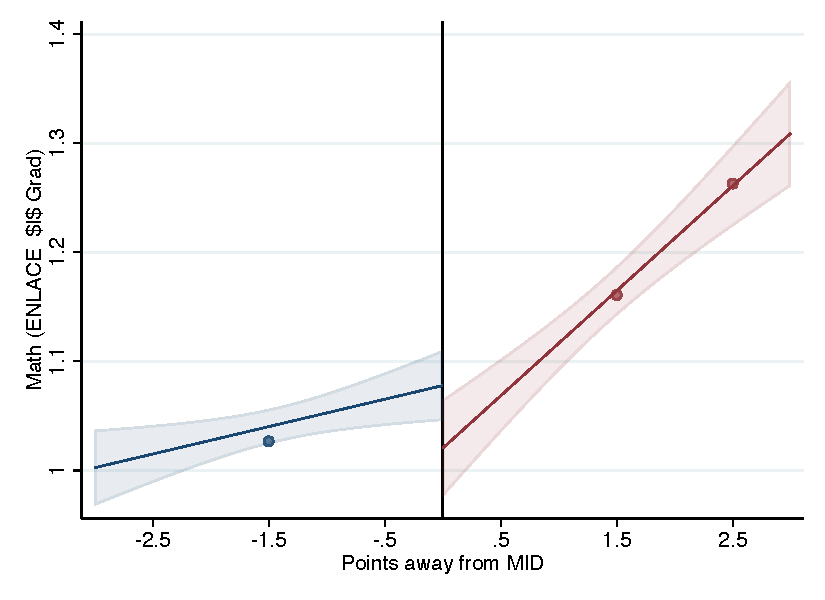
\includegraphics[width=\textwidth]{04_Figures/rd_plot_mid_p_mat_3_IPN3.pdf}
    \end{subfigure}
    
\end{figure}
\end{frame}

\begin{frame}{RD plots of ITT effects for outcomes}
\hyperlink{ITT_rd_plot_IPN}{\beamergotobutton{Back}}
\begin{figure}

    \begin{subfigure}{0.45\textwidth}
        \centering
        \caption{\% Voted (2012) around cutoff}
        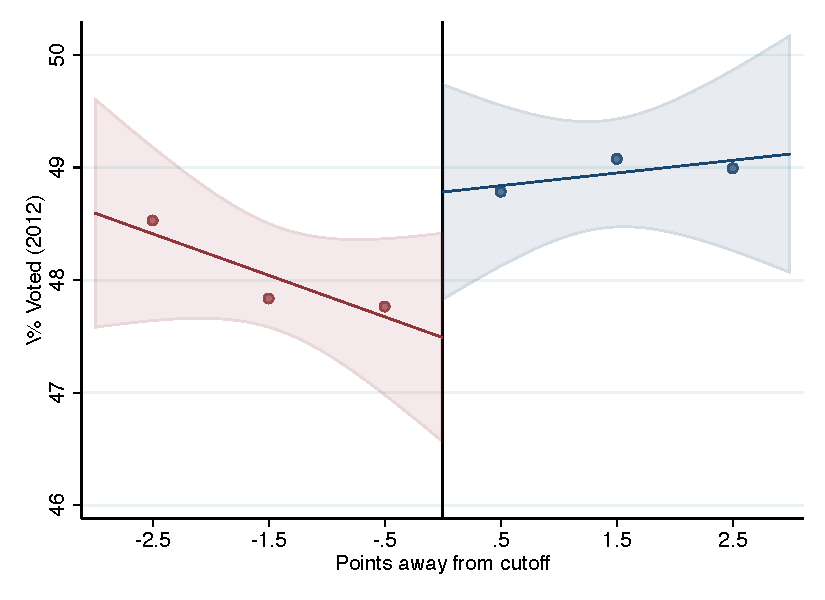
\includegraphics[width=\textwidth]{04_Figures/rd_plot_tau_Voto_Marcado_2012_IPN3.pdf}
    \end{subfigure}
    \begin{subfigure}{0.45\textwidth}
        \centering
        \caption{\% Voted (2012) around MID}
        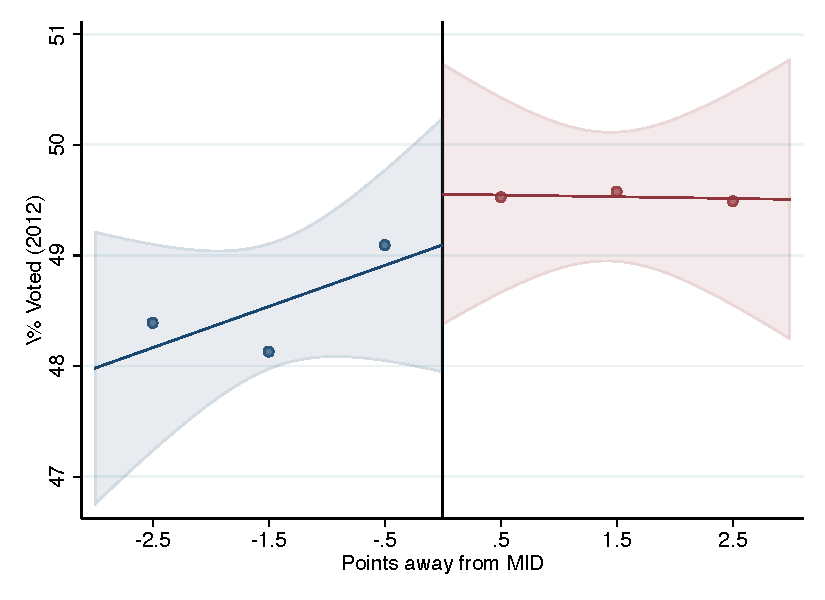
\includegraphics[width=\textwidth]{04_Figures/rd_plot_mid_Voto_Marcado_2012_IPN3.pdf}
    \end{subfigure}
    
\end{figure}
\end{frame}

\begin{frame}{RD plots of ITT effects for outcomes}
\hyperlink{ITT_rd_plot_IPN}{\beamergotobutton{Back}}
\begin{figure}

    \begin{subfigure}{0.45\textwidth}
        \centering
        \caption{\% Voted (2015) around cutoff}
        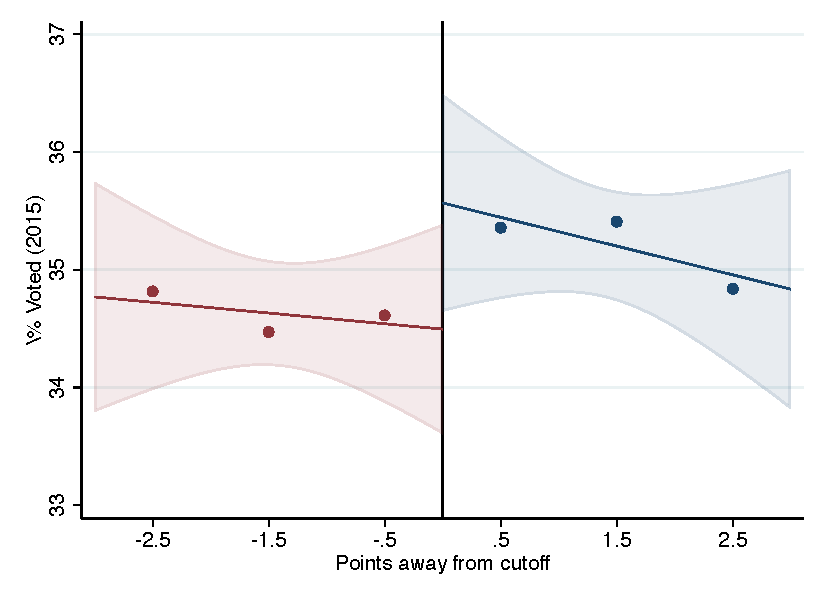
\includegraphics[width=\textwidth]{04_Figures/rd_plot_tau_Voto_Marcado_2015_IPN3.pdf}
    \end{subfigure}
    \begin{subfigure}{0.45\textwidth}
        \centering
        \caption{\% Voted (2015) around MID}
        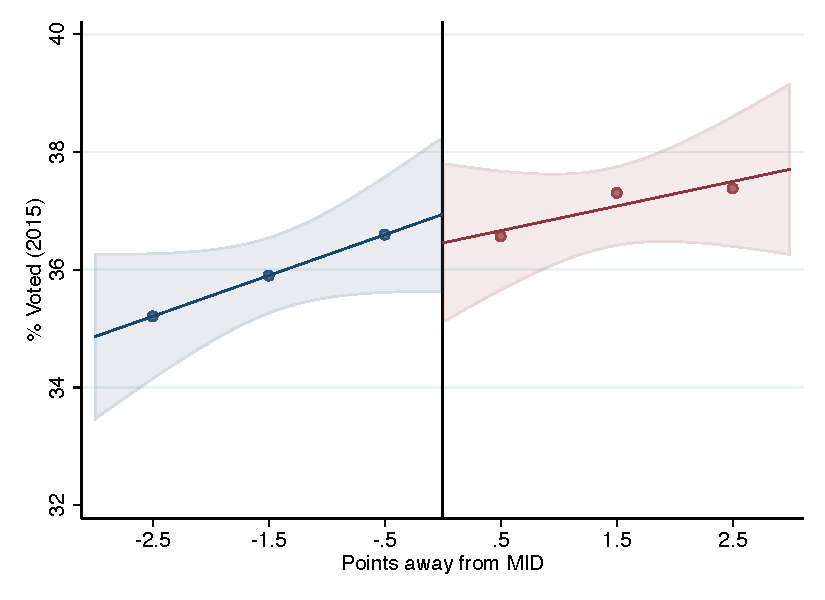
\includegraphics[width=\textwidth]{04_Figures/rd_plot_mid_Voto_Marcado_2015_IPN3.pdf}
    \end{subfigure}
    
\end{figure}
\end{frame}

\begin{frame}{RD plots of ITT effects for outcomes}
\hyperlink{ITT_rd_plot_IPN}{\beamergotobutton{Back}}
\begin{figure}

    \begin{subfigure}{0.45\textwidth}
        \centering
        \caption{\% Voted (2018) around cutoff}
        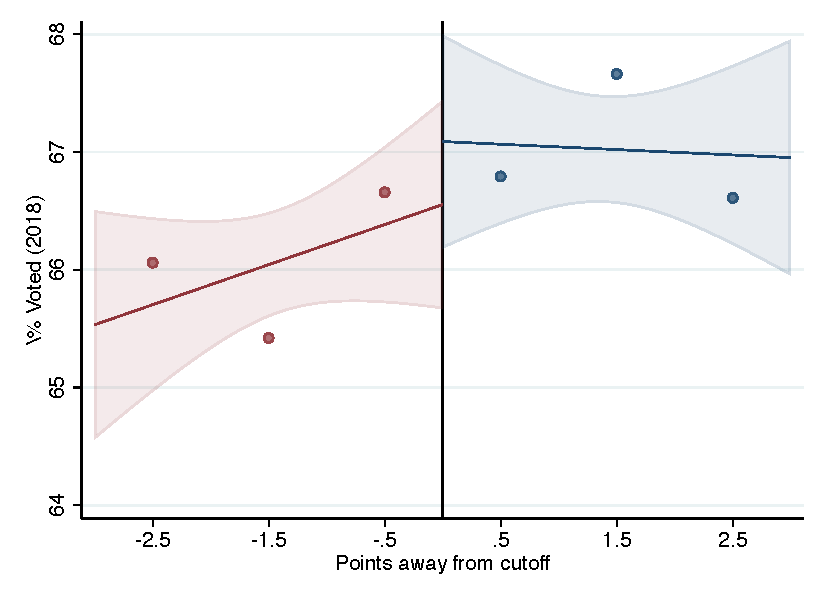
\includegraphics[width=\textwidth]{04_Figures/rd_plot_tau_Voto_Marcado_2018_IPN3.pdf}
    \end{subfigure}
    \begin{subfigure}{0.45\textwidth}
        \centering
        \caption{\% Voted (2018) around MID}
        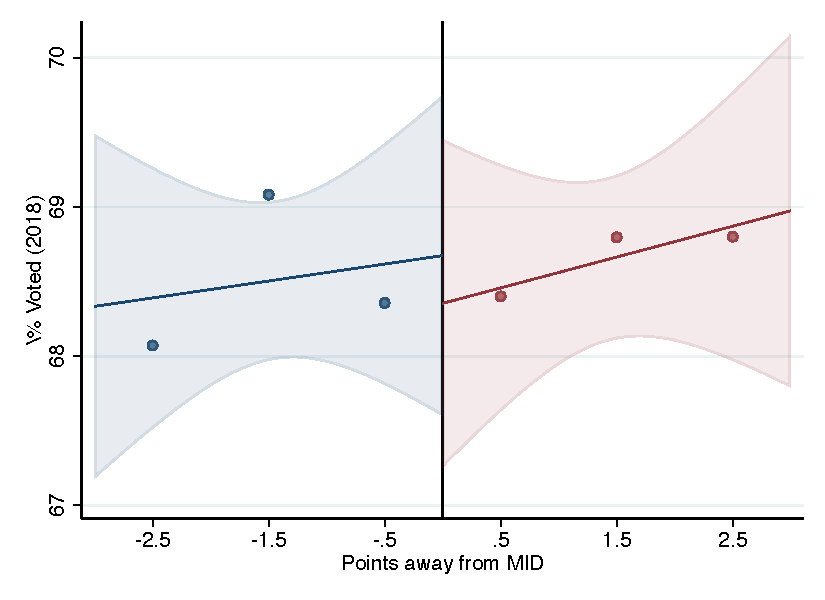
\includegraphics[width=\textwidth]{04_Figures/rd_plot_mid_Voto_Marcado_2018_IPN3.pdf}
    \end{subfigure}
    
\end{figure}
\end{frame}

\begin{frame}{RD plots of ITT effects for outcomes}
\hyperlink{ITT_rd_plot_IPN}{\beamergotobutton{Back}}
\begin{figure}

    \begin{subfigure}{0.45\textwidth}
        \centering
        \caption{\% Crime (INE) around cutoff}
        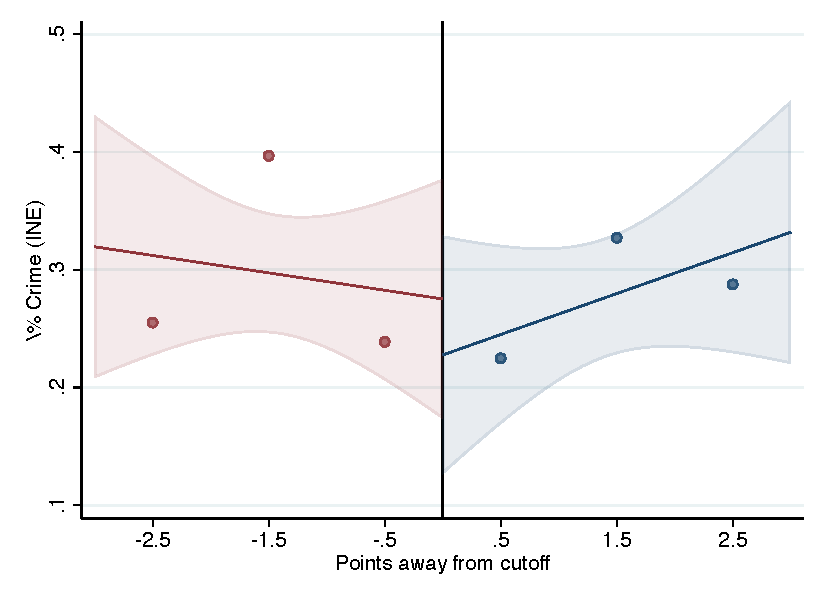
\includegraphics[width=\textwidth]{04_Figures/rd_plot_tau_Suspencion_INE_IPN3.pdf}
    \end{subfigure}
    \begin{subfigure}{0.45\textwidth}
        \centering
        \caption{\% Crime (INE) around MID}
        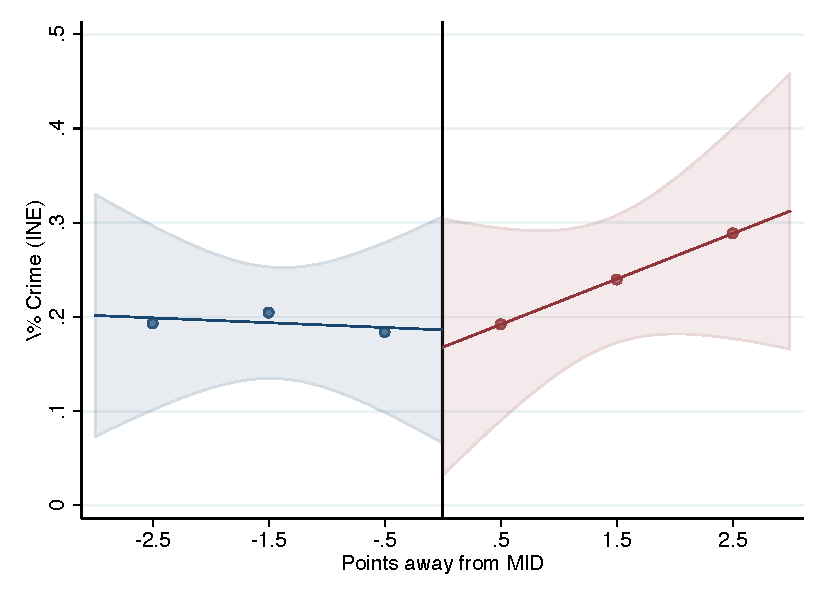
\includegraphics[width=\textwidth]{04_Figures/rd_plot_mid_Suspencion_INE_IPN3.pdf}
    \end{subfigure}
    
\end{figure}
\end{frame}

\begin{frame}{RD plots of ITT effects for outcomes}
\hyperlink{ITT_rd_plot_IPN}{\beamergotobutton{Back}}
\begin{figure}

    \begin{subfigure}{0.45\textwidth}
        \centering
        \caption{\% Death (INE) around cutoff}
        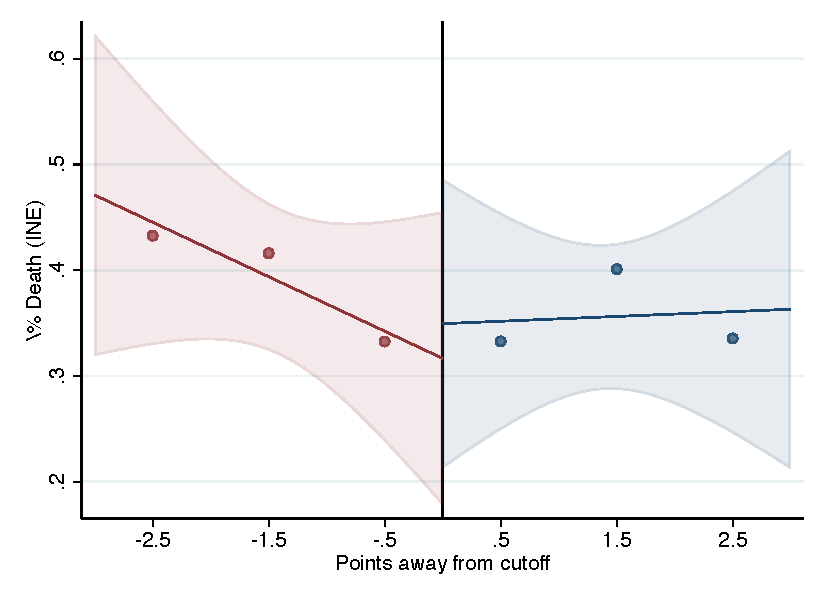
\includegraphics[width=\textwidth]{04_Figures/rd_plot_tau_Death_INE_IPN3.pdf}
    \end{subfigure}
    \begin{subfigure}{0.45\textwidth}
        \centering
        \caption{\% Death (INE) around MID}
        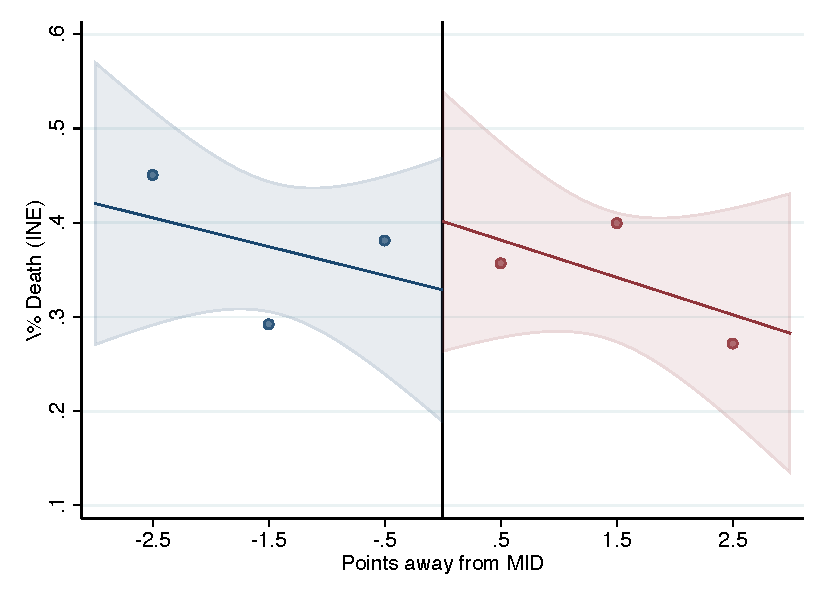
\includegraphics[width=\textwidth]{04_Figures/rd_plot_mid_Death_INE_IPN3.pdf}
    \end{subfigure}
    
\end{figure}
\end{frame}

\begin{frame}{RD plots of ITT effects for outcomes}
\hyperlink{ITT_rd_plot_IPN}{\beamergotobutton{Back}}
\begin{figure}

    \begin{subfigure}{0.45\textwidth}
        \centering
        \caption{\% INE expired around cutoff}
        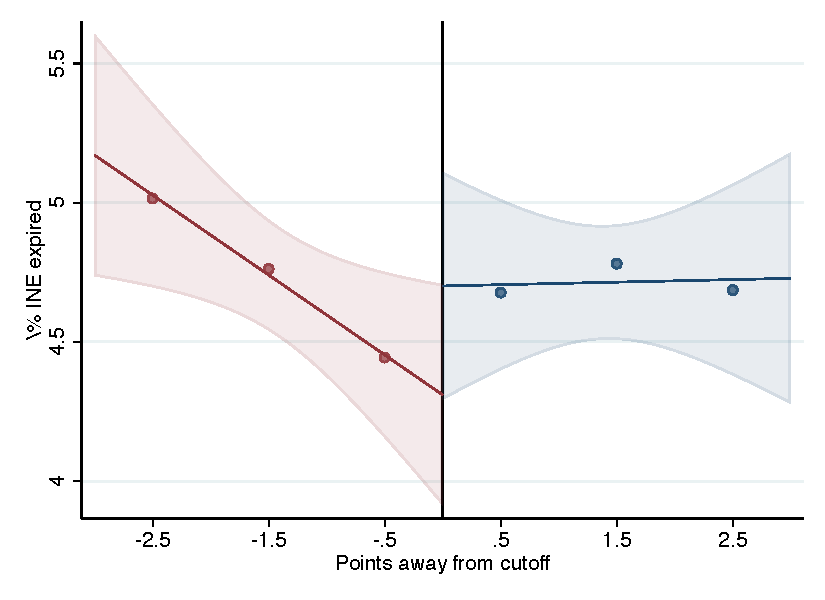
\includegraphics[width=\textwidth]{04_Figures/rd_plot_tau_Expired_INE_IPN3.pdf}
    \end{subfigure}
    \begin{subfigure}{0.45\textwidth}
        \centering
        \caption{\% INE expired around MID}
        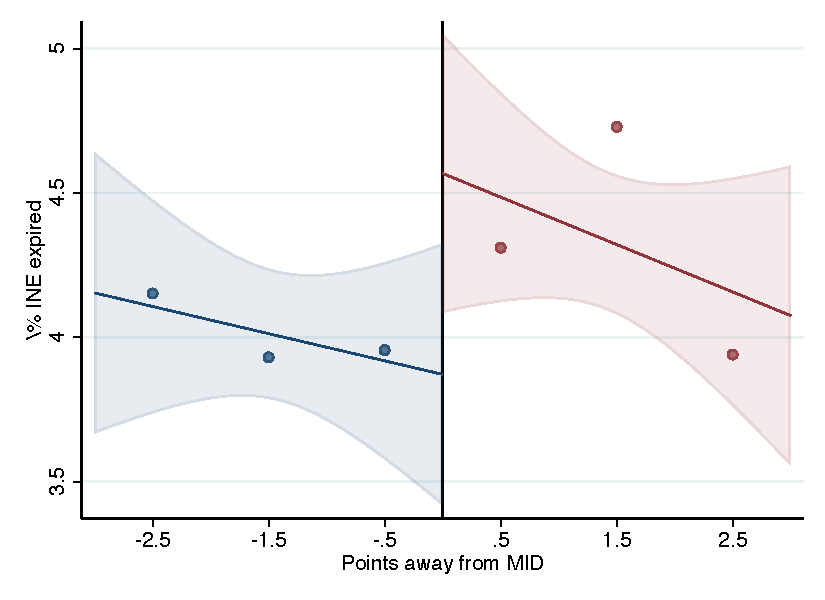
\includegraphics[width=\textwidth]{04_Figures/rd_plot_mid_Expired_INE_IPN3.pdf}
    \end{subfigure}
    
\end{figure}
\end{frame}

\begin{frame}{RD plots of ITT effects for outcomes}
\hyperlink{ITT_rd_plot_IPN}{\beamergotobutton{Back}}
\begin{figure}

    \begin{subfigure}{0.45\textwidth}
        \centering
        \caption{\% Completed HS around cutoff}
        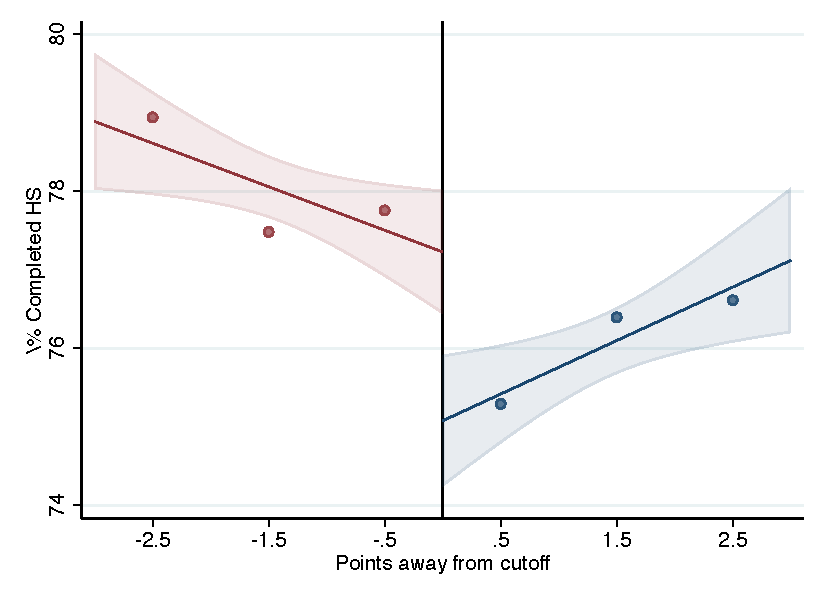
\includegraphics[width=\textwidth]{04_Figures/rd_plot_tau_bachillerato_mas_IPN3.pdf}
    \end{subfigure}
    \begin{subfigure}{0.45\textwidth}
        \centering
        \caption{\% Completed HS around MID}
        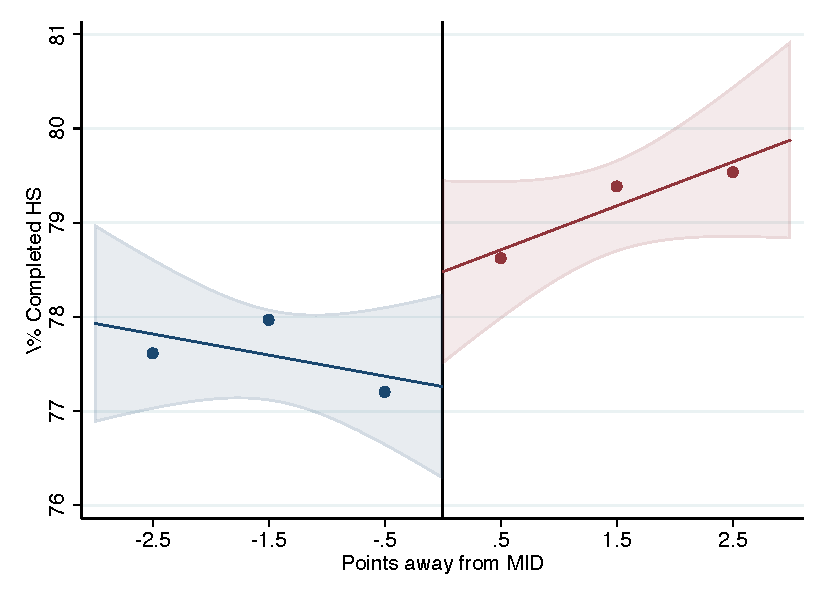
\includegraphics[width=\textwidth]{04_Figures/rd_plot_mid_bachillerato_mas_IPN3.pdf}
    \end{subfigure}
    
\end{figure}
\end{frame}

\begin{frame}{RD plots of ITT effects for outcomes}
\hyperlink{ITT_rd_plot_IPN}{\beamergotobutton{Back}}
\begin{figure}

    \begin{subfigure}{0.45\textwidth}
        \centering
        \caption{\% Post-secondary education around cutoff}
        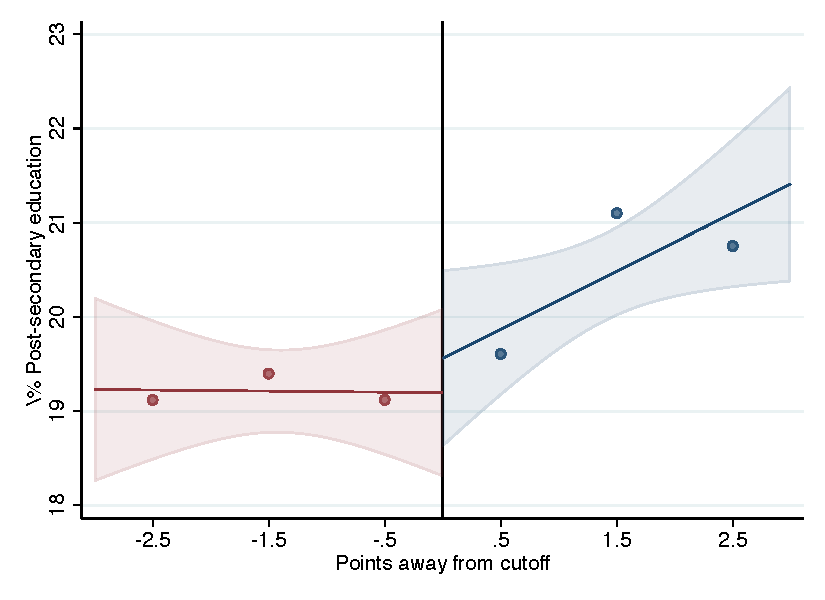
\includegraphics[width=\textwidth]{04_Figures/rd_plot_tau_licenciatura_mas_IPN3.pdf}
    \end{subfigure}
    \begin{subfigure}{0.45\textwidth}
        \centering
        \caption{\% Post-secondary education around MID}
        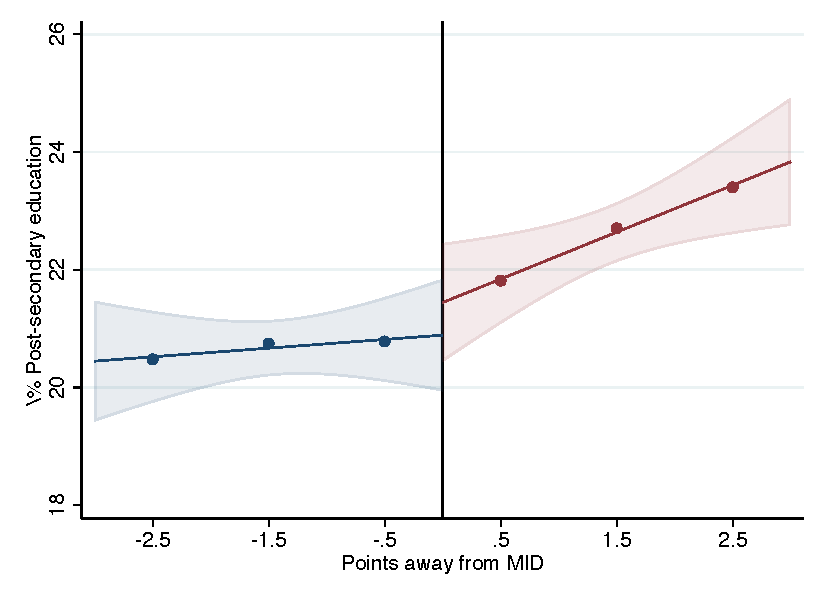
\includegraphics[width=\textwidth]{04_Figures/rd_plot_mid_licenciatura_mas_IPN3.pdf}
    \end{subfigure}
    
\end{figure}
\end{frame}

\begin{frame}{RD plots of ITT effects for outcomes}
\hyperlink{ITT_rd_plot_IPN}{\beamergotobutton{Back}}
\begin{figure}

    \begin{subfigure}{0.45\textwidth}
        \centering
        \caption{\% Unemployed around cutoff}
        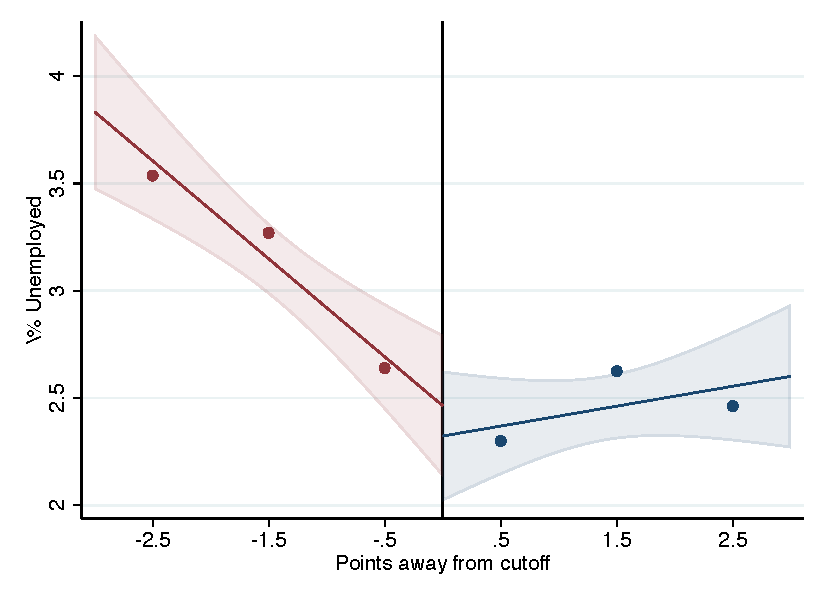
\includegraphics[width=\textwidth]{04_Figures/rd_plot_tau_Unemployed_IPN3.pdf}
    \end{subfigure}
    \begin{subfigure}{0.45\textwidth}
        \centering
        \caption{\% Unemployed around MID}
        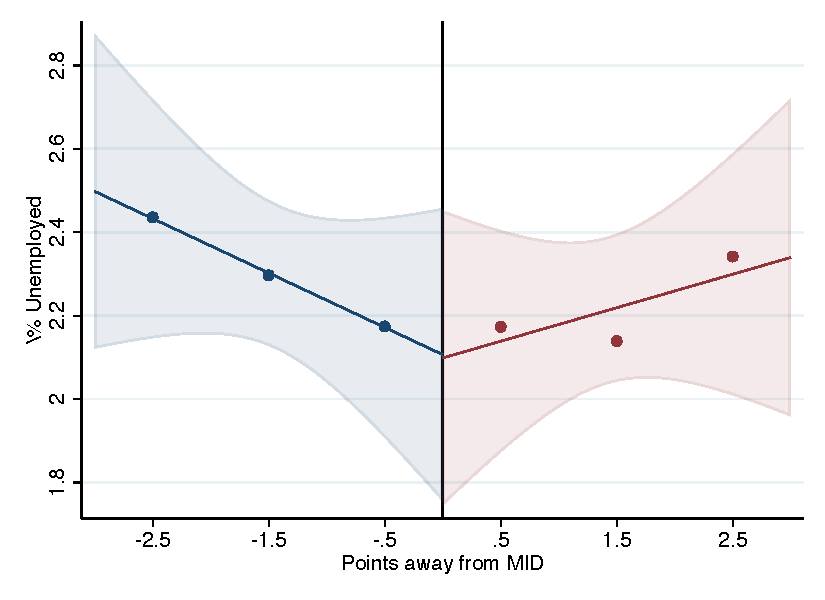
\includegraphics[width=\textwidth]{04_Figures/rd_plot_mid_Unemployed_IPN3.pdf}
    \end{subfigure}
    
\end{figure}
\end{frame}

\begin{frame}{RD plots of ITT effects for outcomes}
\hyperlink{ITT_rd_plot_IPN}{\beamergotobutton{Back}}
\begin{figure}

    \begin{subfigure}{0.45\textwidth}
        \centering
        \caption{\% Housewife around cutoff}
        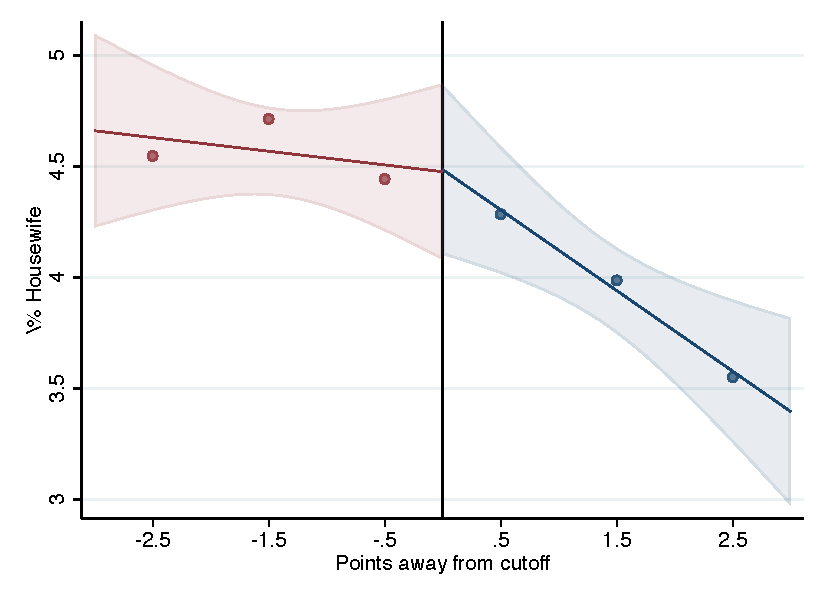
\includegraphics[width=\textwidth]{04_Figures/rd_plot_tau_Housewife_IPN3.pdf}
    \end{subfigure}
    \begin{subfigure}{0.45\textwidth}
        \centering
        \caption{\% Housewife around MID}
        \includegraphics[width=\textwidth]{04_Figures/rd_plot_mid_Housewife_IPN3.pdf}
    \end{subfigure}
    
\end{figure}
\end{frame}


\begin{frame}{RD plots of ITT effects for outcomes}
\hyperlink{ITT_rd_plot_IPN}{\beamergotobutton{Back}}
\begin{figure}

    \begin{subfigure}{0.45\textwidth}
        \centering
        \caption{\% Self-employed around cutoff}
        \includegraphics[width=\textwidth]{04_Figures/rd_plot_tau_Selfemployed_IPN3.pdf}
    \end{subfigure}
    \begin{subfigure}{0.45\textwidth}
        \centering
        \caption{\% Self-employed around MID}
        \includegraphics[width=\textwidth]{04_Figures/rd_plot_mid_Selfemployed_IPN3.pdf}
    \end{subfigure}
    
\end{figure}
\end{frame}

\end{document}